% ====================================================================
% SUPERSEDED. This draft is written against the SYNTHETIC testbed, in which
% the ESG -> distress relationship is INJECTED by the generator at gamma=-4.0.
% Every number in it is from generated data and none of them describe the real
% Bloomberg panel.
%
% The current paper is paper/cresta_real.tex, generated from the pipeline's
% own artefacts by src/generate_paper.py. See paper/README.md.
%
% Kept as the record of the earlier work. Do not cite results from this file.
% ====================================================================
\PassOptionsToPackage{expansion=false}{microtype}
\documentclass[sigconf,anonymous]{acmart}

\usepackage{placeins}
\usepackage{amsmath,amsfonts}
\usepackage{algorithmic}
\usepackage{graphicx}
\usepackage{textcomp}
\usepackage{xcolor}
\usepackage{booktabs}
\usepackage{hyperref}
\usepackage{multirow}
\usepackage{caption}
\usepackage{subcaption}

\AtBeginDocument{%
  \providecommand\BibTeX{{Bib\TeX}}}
  
\makeatletter\@ACM@balancefalse\makeatother

\settopmatter{printacmref=true, printccs=true, printfolios=true}

\setcopyright{acmlicensed}

\acmConference[ICDCN 2027]{28th International Conference on Distributed Computing and Networking}{January 4--7, 2027}{NITK Surathkal, India}
\acmBooktitle{Proceedings of 28th International Conference on Distributed Computing and Networking (ICDCN 2027)}
\copyrightyear{2027}
\acmYear{2027}
\acmDOI{10.1145/nnnnnnn.nnnnnnn}
\acmISBN{978-x-xxxx-xxxx-x/YYYY/MM}

\citestyle{acmnumeric}
\setcitestyle{numbers,square,comma}

\begin{document}

\title{Beyond Circularity: A Forward-Looking Evaluation Framework for ESG-Augmented Corporate Distress Prediction}

\begin{abstract}
Corporate financial distress prediction is central to credit risk management, yet contemporary models frequently achieve near-perfect discrimination scores by exploiting label circularity---a condition in which predictive features share deterministic accounting relationships with the distress label itself. When circularity is present, models learn concurrent accounting identities rather than forward-looking risk signals, yielding performance that does not survive temporal separation.

This paper introduces the Comprehensive Risk Evaluation and Sustainability Tracking Architecture (CRESTA), an evaluation framework that enforces strict temporal separation between predictors and labels ($X_t \to Y_{t+1}$) and ablates features that are circular with respect to the distress definition. To validate the framework's capacity to recover a deliberately injected signal, we constructed a controlled synthetic testbed comprising 60,000 firms over 10~fiscal years (2015--2024). A known Environmental, Social, and Governance (ESG) correlation factor ($\gamma = -4.0$) was embedded in the distress-generation mechanism, providing verifiable ground truth.

Under strict out-of-time evaluation (training: 2015--2022; testing: 2023--2024) on 115,873 test observations containing 264 verified distress events (0.2278\% prevalence), the financial-only baseline (Model~A) achieved an ROC-AUC of 0.5348 and a PR-AUC of 0.0027, while the ESG-augmented model (Model~B) achieved an ROC-AUC of 0.6117 and a PR-AUC of 0.0034. A 2,000-iteration percentile bootstrap yielded $\Delta$AUC~$= +0.0774$ (95\% CI: [$+0.0455$, $+0.1080$]), and SHAP analysis confirmed that the three ESG variables ranked as the top global predictors by mean absolute attribution. These results demonstrate controlled signal recovery after temporal separation and circular-feature ablation; real-world validation on mandated Indian BRSR disclosures remains future work.
\end{abstract}

\begin{CCSXML}
<ccs2012>
   <concept>
       <concept_id>10010147.10010257.10010293.10010294</concept_id>
       <concept_desc>Computing methodologies~Supervised learning by classification</concept_desc>
       <concept_significance>500</concept_significance>
       </concept>
   <concept>
       <concept_id>10010405.10010455.10010460</concept_id>
       <concept_desc>Applied computing~Economics</concept_desc>
       <concept_significance>300</concept_significance>
       </concept>
 </ccs2012>
\end{CCSXML}

\ccsdesc[500]{Computing methodologies~Supervised learning by classification}
\ccsdesc[300]{Applied computing~Economics}

\keywords{Corporate Distress, Label Circularity, ESG Integration, XGBoost, Out-of-Time Testing, SHAP, Partial Dependence, Class Imbalance}

\maketitle

%% ============================================================
%%  1. INTRODUCTION
%% ============================================================
\section{Introduction}

Predicting corporate financial distress---the inability of a firm to meet its debt obligations, potentially leading to default, restructuring, or bankruptcy---is a long-standing challenge in quantitative finance. Accurate forward-looking models inform lending decisions, portfolio risk management, and prudential regulation. Since Altman's pioneering Z-score discriminant model \cite{altman1968}, the field has progressed through logistic regression \cite{ohlson1980}, structural credit models \cite{merton1974}, and contemporary gradient-boosted ensembles \cite{chen2016, ke2017}. Each generation of models has brought higher reported discrimination scores, with recent studies routinely reporting ROC-AUC values above 0.95.

A fundamental flaw undermines many highly cited bankruptcy models. Researchers often construct distress labels from concurrent financial data---for instance, defining a default state as possessing negative equity or an interest coverage ratio falling below~1.0. If these exact metrics subsequently appear as inputs, the model bypasses genuine prediction entirely. Instead, it learns a trivial algebraic identity. We categorize this specific error as \textit{label circularity}, an extreme case of target leakage \cite{sculley2015}. A classifier boasting a 0.99 ROC-AUC because it noticed that liabilities currently outstrip assets has zero forward-looking value. It operates strictly as a concurrent balance sheet auditor. As Rabanser et al.\ \cite{rabanser2019} and Sculley et al.\ \cite{sculley2015} argue regarding technical debt, such structurally compromised architectures invariably break down when confronted with true out-of-time forecasting tasks.

Incorporating Environmental, Social, and Governance (ESG) metrics further complicates model design. Emerging disclosure regimes, notably India's Business Responsibility and Sustainability Reporting (BRSR) mandate, are producing non-financial datasets of unprecedented scale. Finance scholars suggest these disclosures capture long-tail risks---including environmental fines, executive misconduct, or supply chain fragility---months or years before they hit the income statement \cite{friede2015}. Validating this intuition, however, requires a pristine analytical environment. If a researcher trains an algorithm on circular financial ratios, those features will saturate the model's capacity. Any authentic predictive value hidden within the ESG data will be completely overpowered by the concurrent accounting noise.

Despite substantial literature on both distress prediction and ESG integration, fewer studies explicitly isolate whether predictive performance survives the combined treatment of temporal separation, circular-feature removal, and out-of-time evaluation while simultaneously testing a known orthogonal signal. Our study directly confronts this methodological gap.

We propose the Comprehensive Risk Evaluation and Sustainability Tracking Architecture (CRESTA). This pipeline imposes a strict $X_t \to Y_{t+1}$ chronological offset, actively deletes variables sharing definitional overlap with the distress label, and utilizes a simulated testbed to prove it can extract a known ESG signal. Isolating features and shifting timeframes are not novel individually; rather, our contribution is synthesizing these mechanics into a rigorous, verifiable laboratory setting. The investigation centers on three questions:

\begin{itemize}
    \item \textbf{RQ1:} How sharply do discrimination scores drop when we strip out circular accounting predictors?
    \item \textbf{RQ2:} Can a model isolate a mathematical ESG factor relying solely on clean, lagged features?
    \item \textbf{RQ3:} What happens to precision, recall, and perceived accuracy when forecasting events at the extreme margins of probability?
\end{itemize}

The paper makes four distinct contributions:
\begin{enumerate}
    \item A diagnostic framework measuring exactly how much performance inflation stems from contemporaneous target leakage.
    \item Empirical proof that an orthogonal ESG correlation factor remains detectable ($\Delta$AUC $= +0.0774$, 95\% CI: [$+0.0455$, $+0.1080$]) even under severe temporal and feature restrictions.
    \item A stress-test of classification metrics at a 0.2278\% test prevalence, proving that optimizing for 98\% accuracy results in missing almost all true defaults.
    \item SHAP-derived verification that the ESG features are driving predictions independently, mirroring the initial simulation design.
\end{enumerate}


%% ============================================================
%%  2. RELATED WORK
%% ============================================================
\section{Related Work}

\subsection{Classical Financial Distress Prediction}
Altman's \cite{altman1968} five-ratio Z-score, developed using multiple discriminant analysis on manufacturing firms, remains one of the most widely cited default prediction models in practice. Ohlson \cite{ohlson1980} advanced the methodology by applying logistic regression, producing probabilistic default estimates that relaxed the strict distributional assumptions of discriminant analysis. Structural approaches rooted in the Black--Scholes--Merton framework \cite{merton1974} recast corporate equity as a call option on the firm's asset value, deriving a \textit{distance-to-default} metric from the firm's asset volatility and leverage. While these classical models offer interpretability and theoretical grounding, they assume linear or log-linear relationships between predictors and default risk. They also rely on small feature sets and static specifications, limiting their capacity to capture the non-linear, multi-dimensional interactions that characterize modern credit risk \cite{jones2017}.

\subsection{Machine Learning for Financial Distress}
Machine learning fundamentally changed credit modeling by handling vast, non-linear feature matrices. Ensembles based on decision trees---notably XGBoost \cite{chen2016} and LightGBM \cite{ke2017}---routinely beat classical logistic regression and discriminant analysis on structured financial tasks. Both large-scale algorithm tournaments \cite{lessmann2015} and focused bankruptcy studies \cite{barboza2017} confirm this edge, with support vector machines offering similarly strong results \cite{bellotti2009}.

However, feeding hundreds of variables into high-capacity algorithms invites severe methodological danger. In distress prediction, \textit{label circularity} stands out as the most damaging error. When researchers build a label using time~$t$ ratios, then feed those same ratios into an XGBoost model, the algorithm stops predicting and starts memorizing algebra. This differs from classic temporal leakage (peeking into the future). Circularity happens in the present tense: the inputs and the target are practically synonyms. Sculley et al.\ \cite{sculley2015} famously cataloged how these hidden data loops rot production software. Later, Rabanser et al.\ \cite{rabanser2019} demonstrated that flawless cross-validation scores routinely hide complete breakdowns in real-world generalization.

\subsection{ESG and Financial Performance}
Friede et al.\ \cite{friede2015} conducted a meta-analysis aggregating more than 2,000 empirical studies and found a predominantly positive relationship between high ESG scores and corporate financial performance. The hypothesis that ESG disclosures capture long-tail risks not reflected in concurrent financial ratios---regulatory exposure, governance failures, climate transition risk---has attracted growing institutional interest \cite{bassen2006}. However, the literature remains heterogeneous. Effect sizes vary across sectors, geographies, and ESG pillars, and the causal direction of the ESG--performance relationship is debated. Testing whether ESG data provides an \textit{orthogonal} risk signal for distress prediction requires separating it from the circular financial features that dominate most existing models.

\subsection{Data Integrity and Temporal Validity}
Credit risk researchers have long insisted on out-of-time validation \cite{lessmann2015, bellotti2009}, a principle forcefully restated in recent machine learning bankruptcy literature \cite{barboza2017}. Jones and colleagues \cite{jones2017} explicitly warn against using randomized cross-validation for rating classifiers, demanding chronological splits instead. Zooming out to general computer science, Sculley et al.\ \cite{sculley2015} mapped out the disastrous effects of data leakage, and Rabanser et al.\ \cite{rabanser2019} built frameworks to catch it. Financial distress models sit directly at the intersection of these warnings, as sloppy target construction inevitably breeds fatal contemporaneous overlap between what the model sees and what it predicts.

\subsection{Explainability in Financial Models}
Lundberg and Lee \cite{lundberg2017} introduced SHAP (SHapley Additive exPlanations), which allocates each feature's marginal contribution to individual predictions based on cooperative game theory. In the context of ESG signal evaluation, explainability serves a specific purpose: it allows verification that ESG features contribute independently to the model's predictions rather than serving as proxies for correlated financial or size variables.

\subsection{Research Gap}
Existing distress prediction studies seldom verify whether their reported performance survives the combined treatment of temporal separation, circular-feature removal, and strict out-of-time evaluation. Studies integrating ESG data rarely test whether the ESG signal remains detectable once circular financial features are ablated. CRESTA addresses this gap by providing a controlled synthetic environment in which a known ESG signal is injected, the pipeline is subjected to circularity controls, and signal recovery is measured under strict temporal evaluation.


%% ============================================================
%%  3. METHODOLOGY
%% ============================================================
\section{Methodology}

\subsection{Pipeline Architecture}
The CRESTA pipeline consists of sequential stages: synthetic data generation, quality gating, feature engineering, circular-feature ablation, temporal target construction, out-of-time train--test split, model training, evaluation, and post-hoc explainability analysis. Figure~\ref{fig_arch} illustrates the end-to-end architecture.

\begin{figure}[htbp]
\centerline{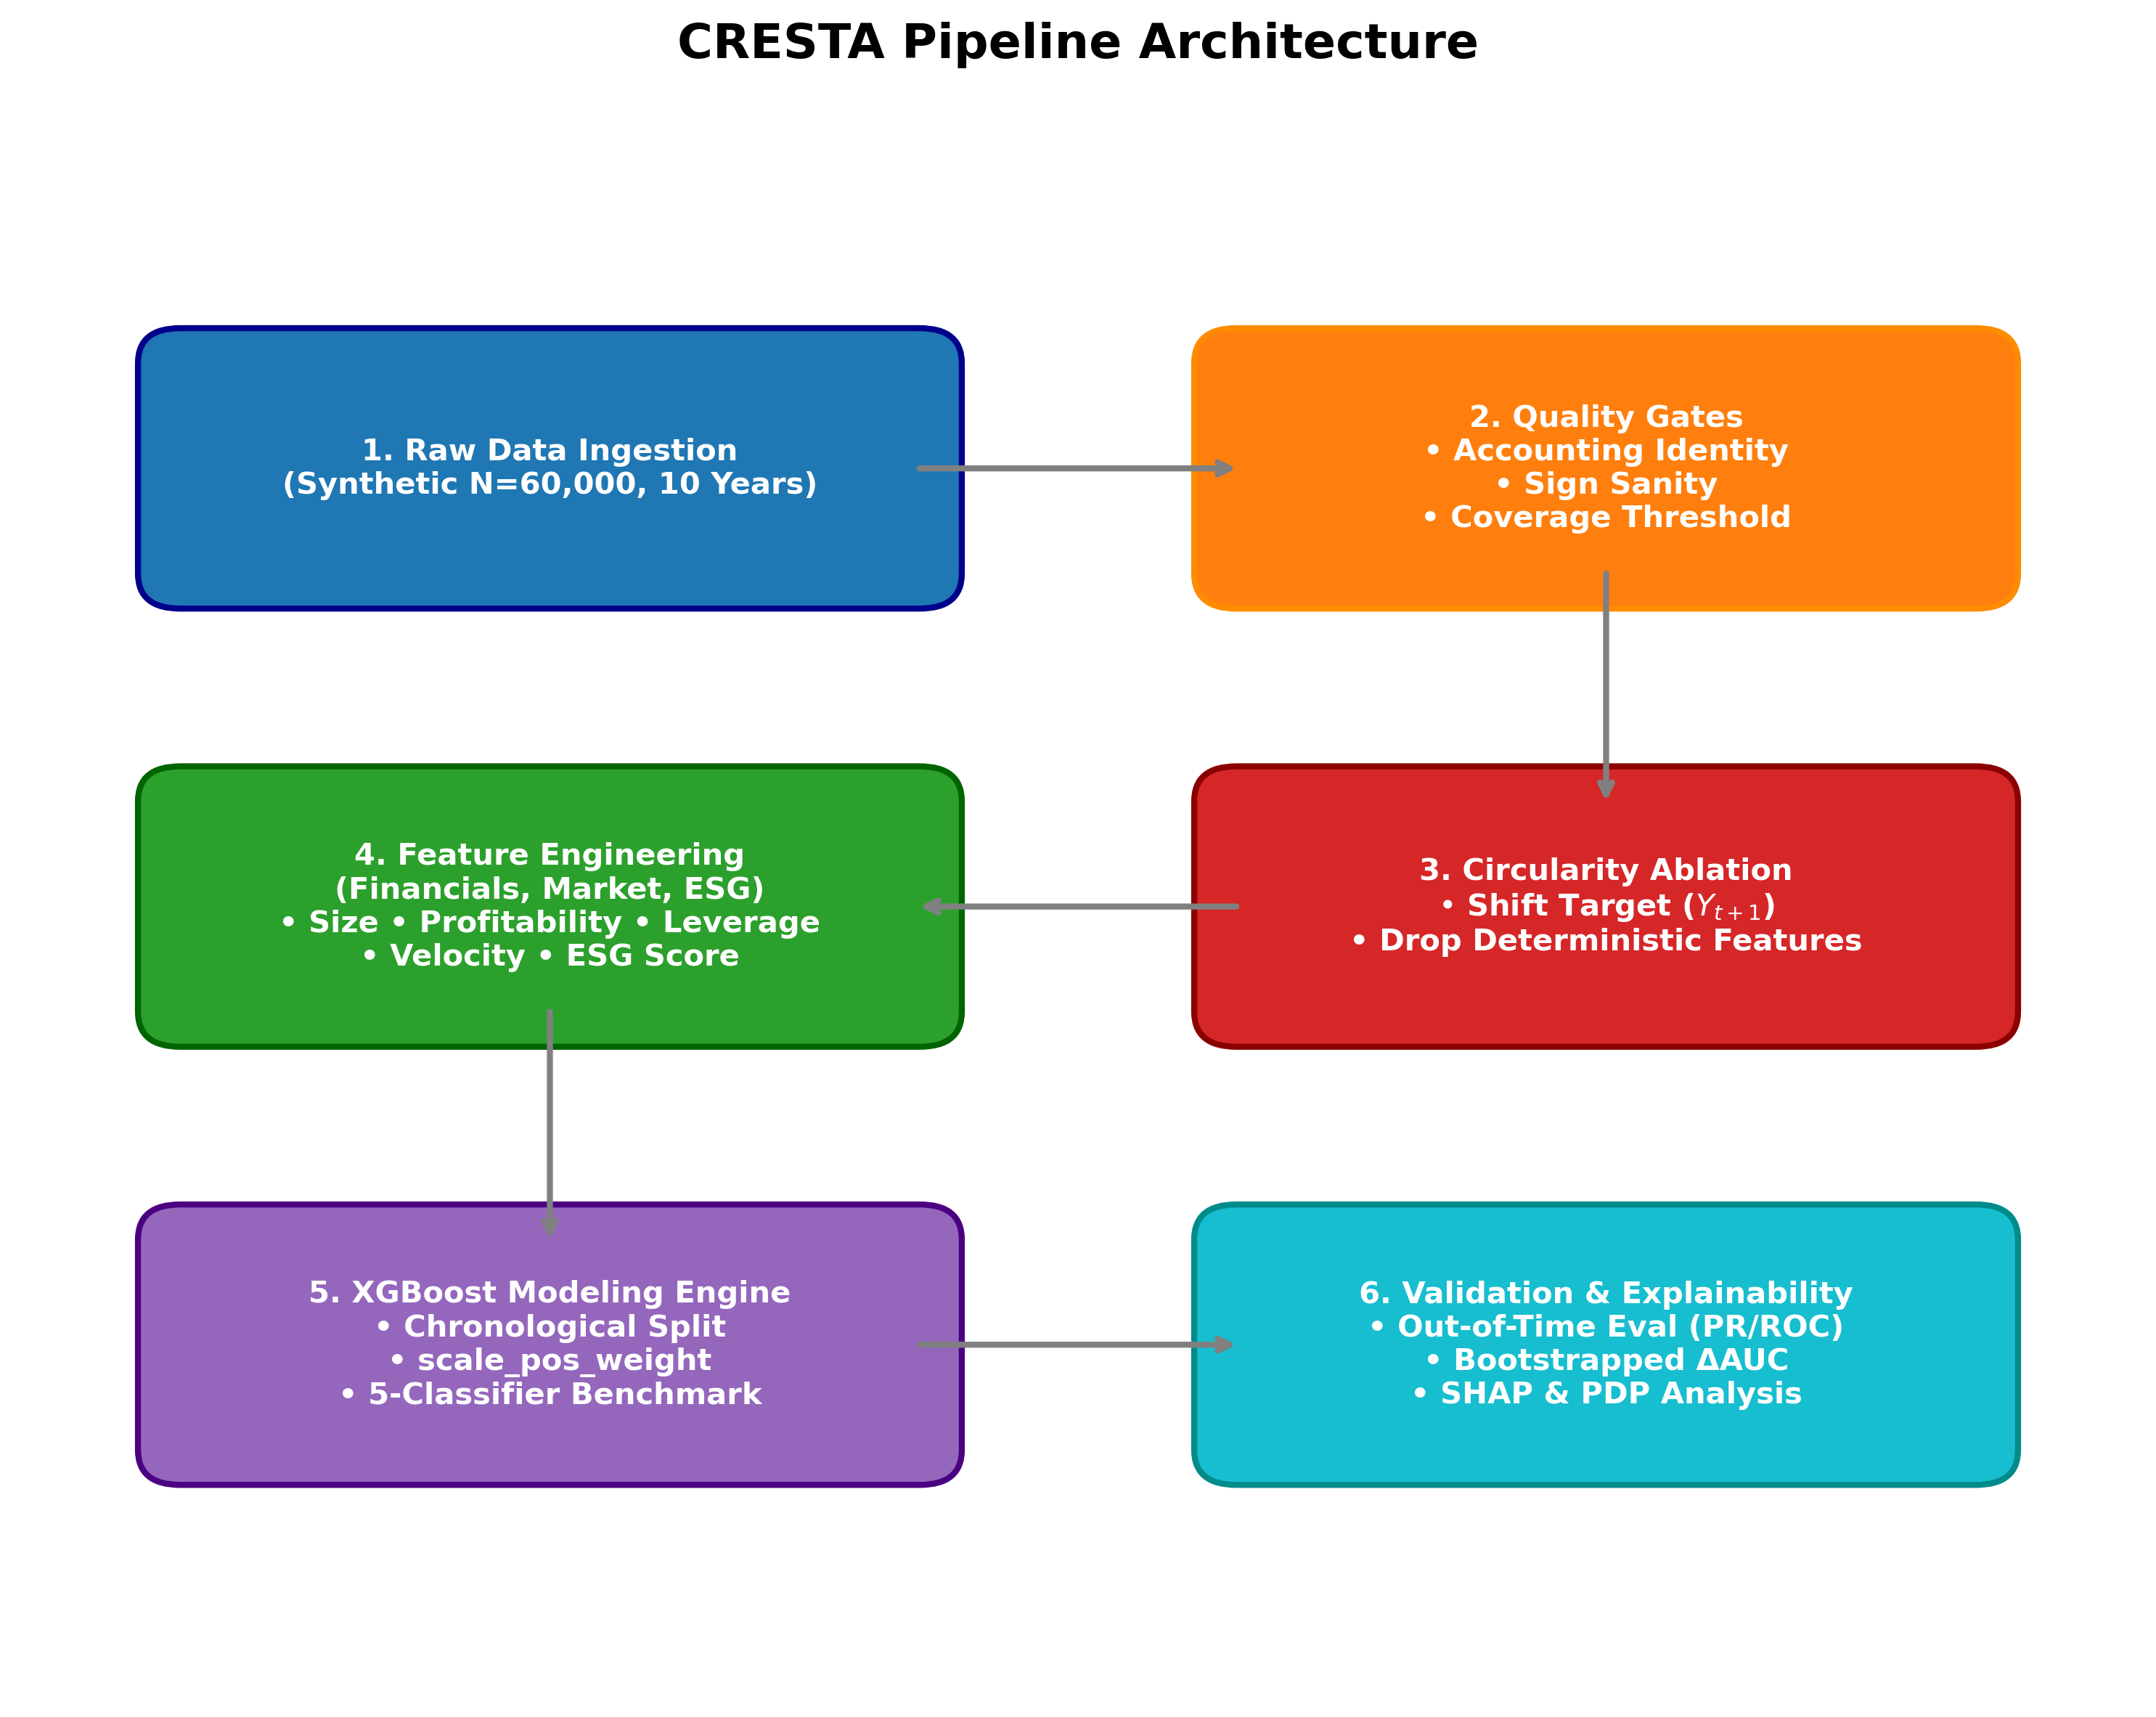
\includegraphics[width=\linewidth]{reports/figures/cresta_architecture.png}}
\caption{CRESTA pipeline architecture. Data flows from generation through quality gating, feature engineering, circular ablation, temporal target construction, out-of-time splitting, model training, and evaluation with post-hoc explainability.}
\label{fig_arch}
\end{figure}

\subsection{Synthetic Panel Generation}
To conduct a controlled experiment, we needed a dataset where the true underlying relationships were indisputable. We wrote a simulation script (locked to random seed 42) to generate a decade of financial records (2015--2024) for 60,000 fictional corporations. The goal was to replicate the messy statistical reality of global equities while secretly embedding a verifiable ESG distress shield into the math.

We mapped the firms into 11 GICS sector buckets using historically accurate weightings. The starting financial position of every entity relied on three foundational parameters:
\begin{itemize}
    \item \textbf{Size:} We drew starting log-assets from a $\mathcal{N}(12.0, 1.5)$ distribution.
    \item \textbf{Profitability:} We assigned baseline ROA utilizing $\mathcal{N}(0.08, 0.04)$.
    \item \textbf{Leverage:} We allocated initial debt burdens from $\mathcal{N}(0.6, 0.3)$.
\end{itemize}

Companies do not remain static, so we evolved their financials longitudinally. We drove market capitalization via standard Geometric Brownian Motion (GBM):
\begin{equation}
    dM_{i,t} = \mu_i M_{i,t} \, dt + \sigma_i M_{i,t} \, dW_{i,t}
\end{equation}
fixing individual drift ($\mu_i$) at 0.05 and stock volatility ($\sigma_i$) at 0.1. Because corporate profits famously regress to the mean, we forced ROA to follow a first-order autoregressive AR(1) path, adding a 0.02 standard deviation shock to each period:
\begin{equation}
    ROA_{i,t} = c + \phi \, ROA_{i,t-1} + \epsilon_{i,t}, \quad \epsilon_{i,t} \sim \mathcal{N}(0, \sigma_\epsilon^2)
\end{equation}

Finally, we coded a strict survivorship rule. If a simulated business fails during year~$t$, the script permanently ejects it from the ledger for years $t+1$ and beyond. The total row count drops continuously as the decade progresses, replicating the attrition of a live stock market.

\subsection{Distress-Generation Mechanism}
The occurrence of a distress event for firm $i$ was governed by a logistic function mapping latent risk factors to a distress probability:
\begin{equation}
    z_i = -2.0 \cdot \text{profit}_i + 0.5 \cdot \text{leverage}_i + \gamma \cdot \frac{\text{base\_esg}_i}{100}
    \label{eq:zscore}
\end{equation}
\begin{equation}
    p_i = \frac{1}{1 + \exp(-(z_i - 2.0))}
    \label{eq:logistic}
\end{equation}
where $\gamma = -4.0$ is the injected ESG distress uplift. A firm experiences distress if a uniform random draw falls below~$p_i$. The division by~100 in Equation~\ref{eq:zscore} means that the effective coefficient per one raw ESG-score unit is $-4.0 / 100 = -0.04$. This parameter structurally guarantees that, holding financial shocks constant, firms with higher latent ESG scores have lower log-odds of distress.

\subsection{ESG Observation Model}
The latent \texttt{base\_esg} score is not directly observed. Instead, noisy observable scores are generated:
\begin{equation}
    e\_score_i = \text{clip}\bigl(\text{base\_esg}_i + \epsilon_i, \; 0, \; 100\bigr), \quad \epsilon_i \sim \mathcal{N}(0, 3)
    \label{eq:esg_obs}
\end{equation}
Independent noise draws produce \texttt{s\_score} and \texttt{g\_score}. Carbon intensity is computed as a function of firm size and environmental score: $\texttt{carbon\_intensity}_i = (\text{total\_assets}_i / 10^6) \times (100 - e\_score_i) \times U(0.8, 1.2)$.

\subsection{Theoretical-to-Empirical Coefficient Mapping}
Because the observable \texttt{e\_score} contains additive Gaussian noise ($\sigma = 3$) relative to \texttt{base\_esg} ($\sigma \approx 15$), classical measurement-error attenuation predicts that a logistic regression on the observed scores will recover a coefficient smaller in magnitude than the true $-0.04$:
\begin{equation}
    \hat{\beta} \approx -0.04 \times \frac{\sigma^2_{\text{signal}}}{\sigma^2_{\text{signal}} + \sigma^2_{\text{noise}}} = -0.04 \times \frac{225}{234} \approx -0.0385
\end{equation}
Our 5-stage signal diagnostic (Section~\ref{sec:signal_diag}) recovers a coefficient of approximately $-0.035$, which is consistent with this theoretical prediction after accounting for boundary clipping, sector-level ESG adjustments, and the linear approximation of a nonlinear data-generating process. We describe this relationship as \textit{theoretical coefficient mapping and empirical recovery}, not as proof.

\begin{figure}[htbp]
\centerline{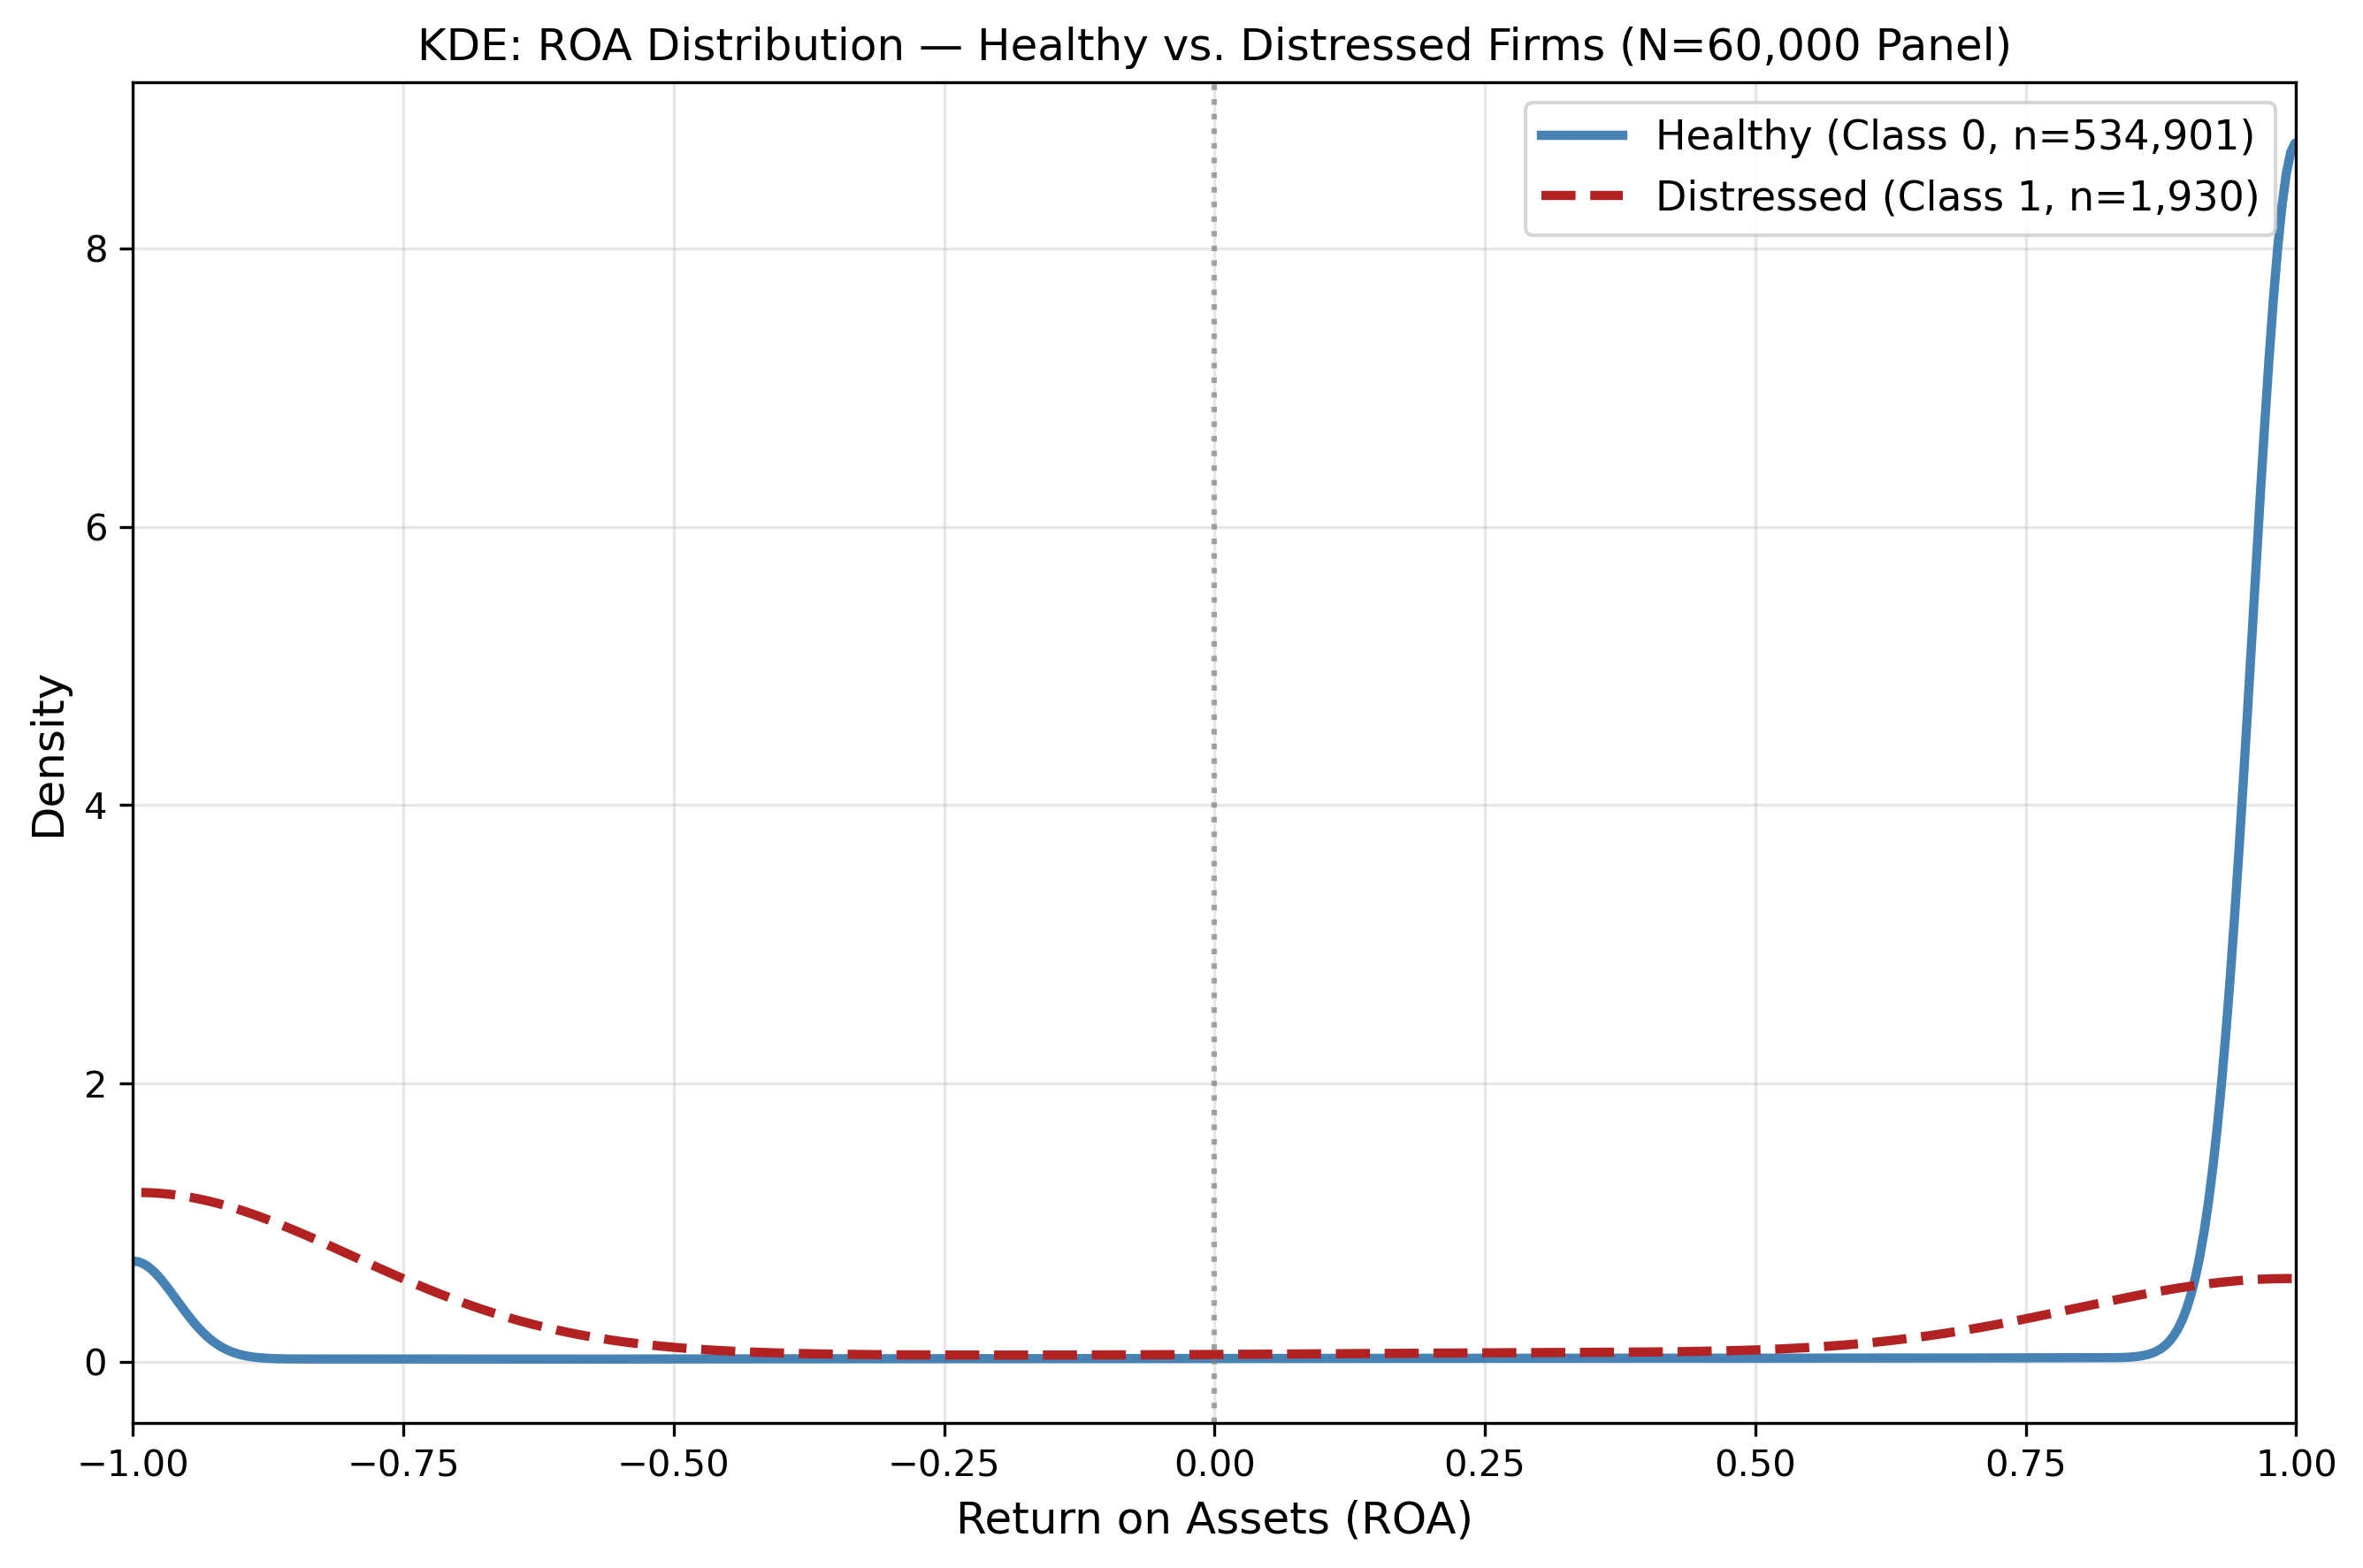
\includegraphics[width=\linewidth]{reports/figures/class_distribution.png}}
\caption{Kernel density estimation comparing the distribution of Return on Assets (ROA) between healthy (Class~0) and distressed (Class~1) firms. The leftward shift of the distressed distribution confirms that the stochastic generation correctly reflects the profitability shock associated with distress events.}
\label{fig_dist}
\end{figure}

Figure~\ref{fig_dist} confirms that the synthetic generation produces the expected distributional separation: distressed firms exhibit a left-shifted ROA distribution relative to healthy firms, reflecting the profitability shock embedded in the generation mechanism.

\subsection{Quality Control}
Prior to feature extraction, we scrubbed the 594,392 simulated records using a sequential seven-stage filter:

\begin{enumerate}
    \item \textbf{Primary Key:} We dropped any row lacking a clean ticker and year pair, resolving index collisions.
    \item \textbf{Accounting Identity:} We computed the gap between assets and total capital (liabilities plus equity). If the mismatch exceeded 2\%, we flagged the row but kept the data intact.
    \item \textbf{Sign Sanity:} Negative or zero total assets are impossible under normal accounting. We hard-deleted exactly 5,943 rows failing this logic check.
    \item \textbf{Range Plausibility:} We stamped extreme outliers in interest coverage and profitability with warning indicators.
    \item \textbf{Coverage:} We audited seven critical financial metrics for NaN values. We discovered 2,097 rows suffering from severe data sparsity (missing >30\%). Rather than dropping them, we deliberately passed them to the XGBoost engine to test its native missing-value handling.
    \item \textbf{Temporal Continuity:} We mapped reporting gaps, raising alerts for firms that vanished and reappeared across spans wider than 24 months.
    \item \textbf{Scale Sanity:} We flagged anomalous Altman Z$''$ computations drifting beyond $\pm$50.
\end{enumerate}

After gating, 588,449 firm-year observations remained. The arithmetic is exact: $594{,}392 - 5{,}943 = 588{,}449$.

\subsection{Feature Engineering}
The pipeline generates 44 engineered features organized into analytical blocks:

\begin{itemize}
    \item \textbf{Leverage \& Solvency:} equity-to-assets, debt-to-assets, net-debt-to-EBITDA proxy, working-capital-to-assets.
    \item \textbf{Liquidity:} current ratio, conservative current ratio.
    \item \textbf{Profitability:} ROA, EBIT margin, net profit margin, CFO-to-assets, CFO-to-debt, asset turnover, EBIT-to-assets, retained-earnings-to-assets.
    \item \textbf{Classical Composite:} Altman Z$''$ (double prime), Altman EMS score, and associated diagnostic flags.
    \item \textbf{Temporal Dynamics:} year-over-year changes in ROA, interest coverage, liabilities-to-assets, Altman~Z; three-year Altman Z trend; consecutive loss years; consecutive IC-below-1 years; revenue growth.
    \item \textbf{Size \& Controls:} log total assets, log market capitalization, financials-sector indicator, equity volatility.
    \item \textbf{ESG:} \texttt{e\_score}, \texttt{s\_score}, \texttt{g\_score}, \texttt{carbon\_intensity}.
\end{itemize}

\subsection{Circular-Feature Ablation}
Six features were identified as circular with respect to common distress definitions and permanently removed from the model input: \texttt{interest\_coverage} (and its capped and below-1 flag derivatives), \texttt{X4\_equity\_to\_liabilities}, \texttt{liabilities\_to\_assets}, and \texttt{negative\_equity\_flag}. After ablation, 38 features remained as final model inputs. Throughout this paper, we distinguish between 44 engineered features (the output of feature engineering), 6 circular features ablated, and 38 final model-input features.

\begin{figure}[htbp]
\centerline{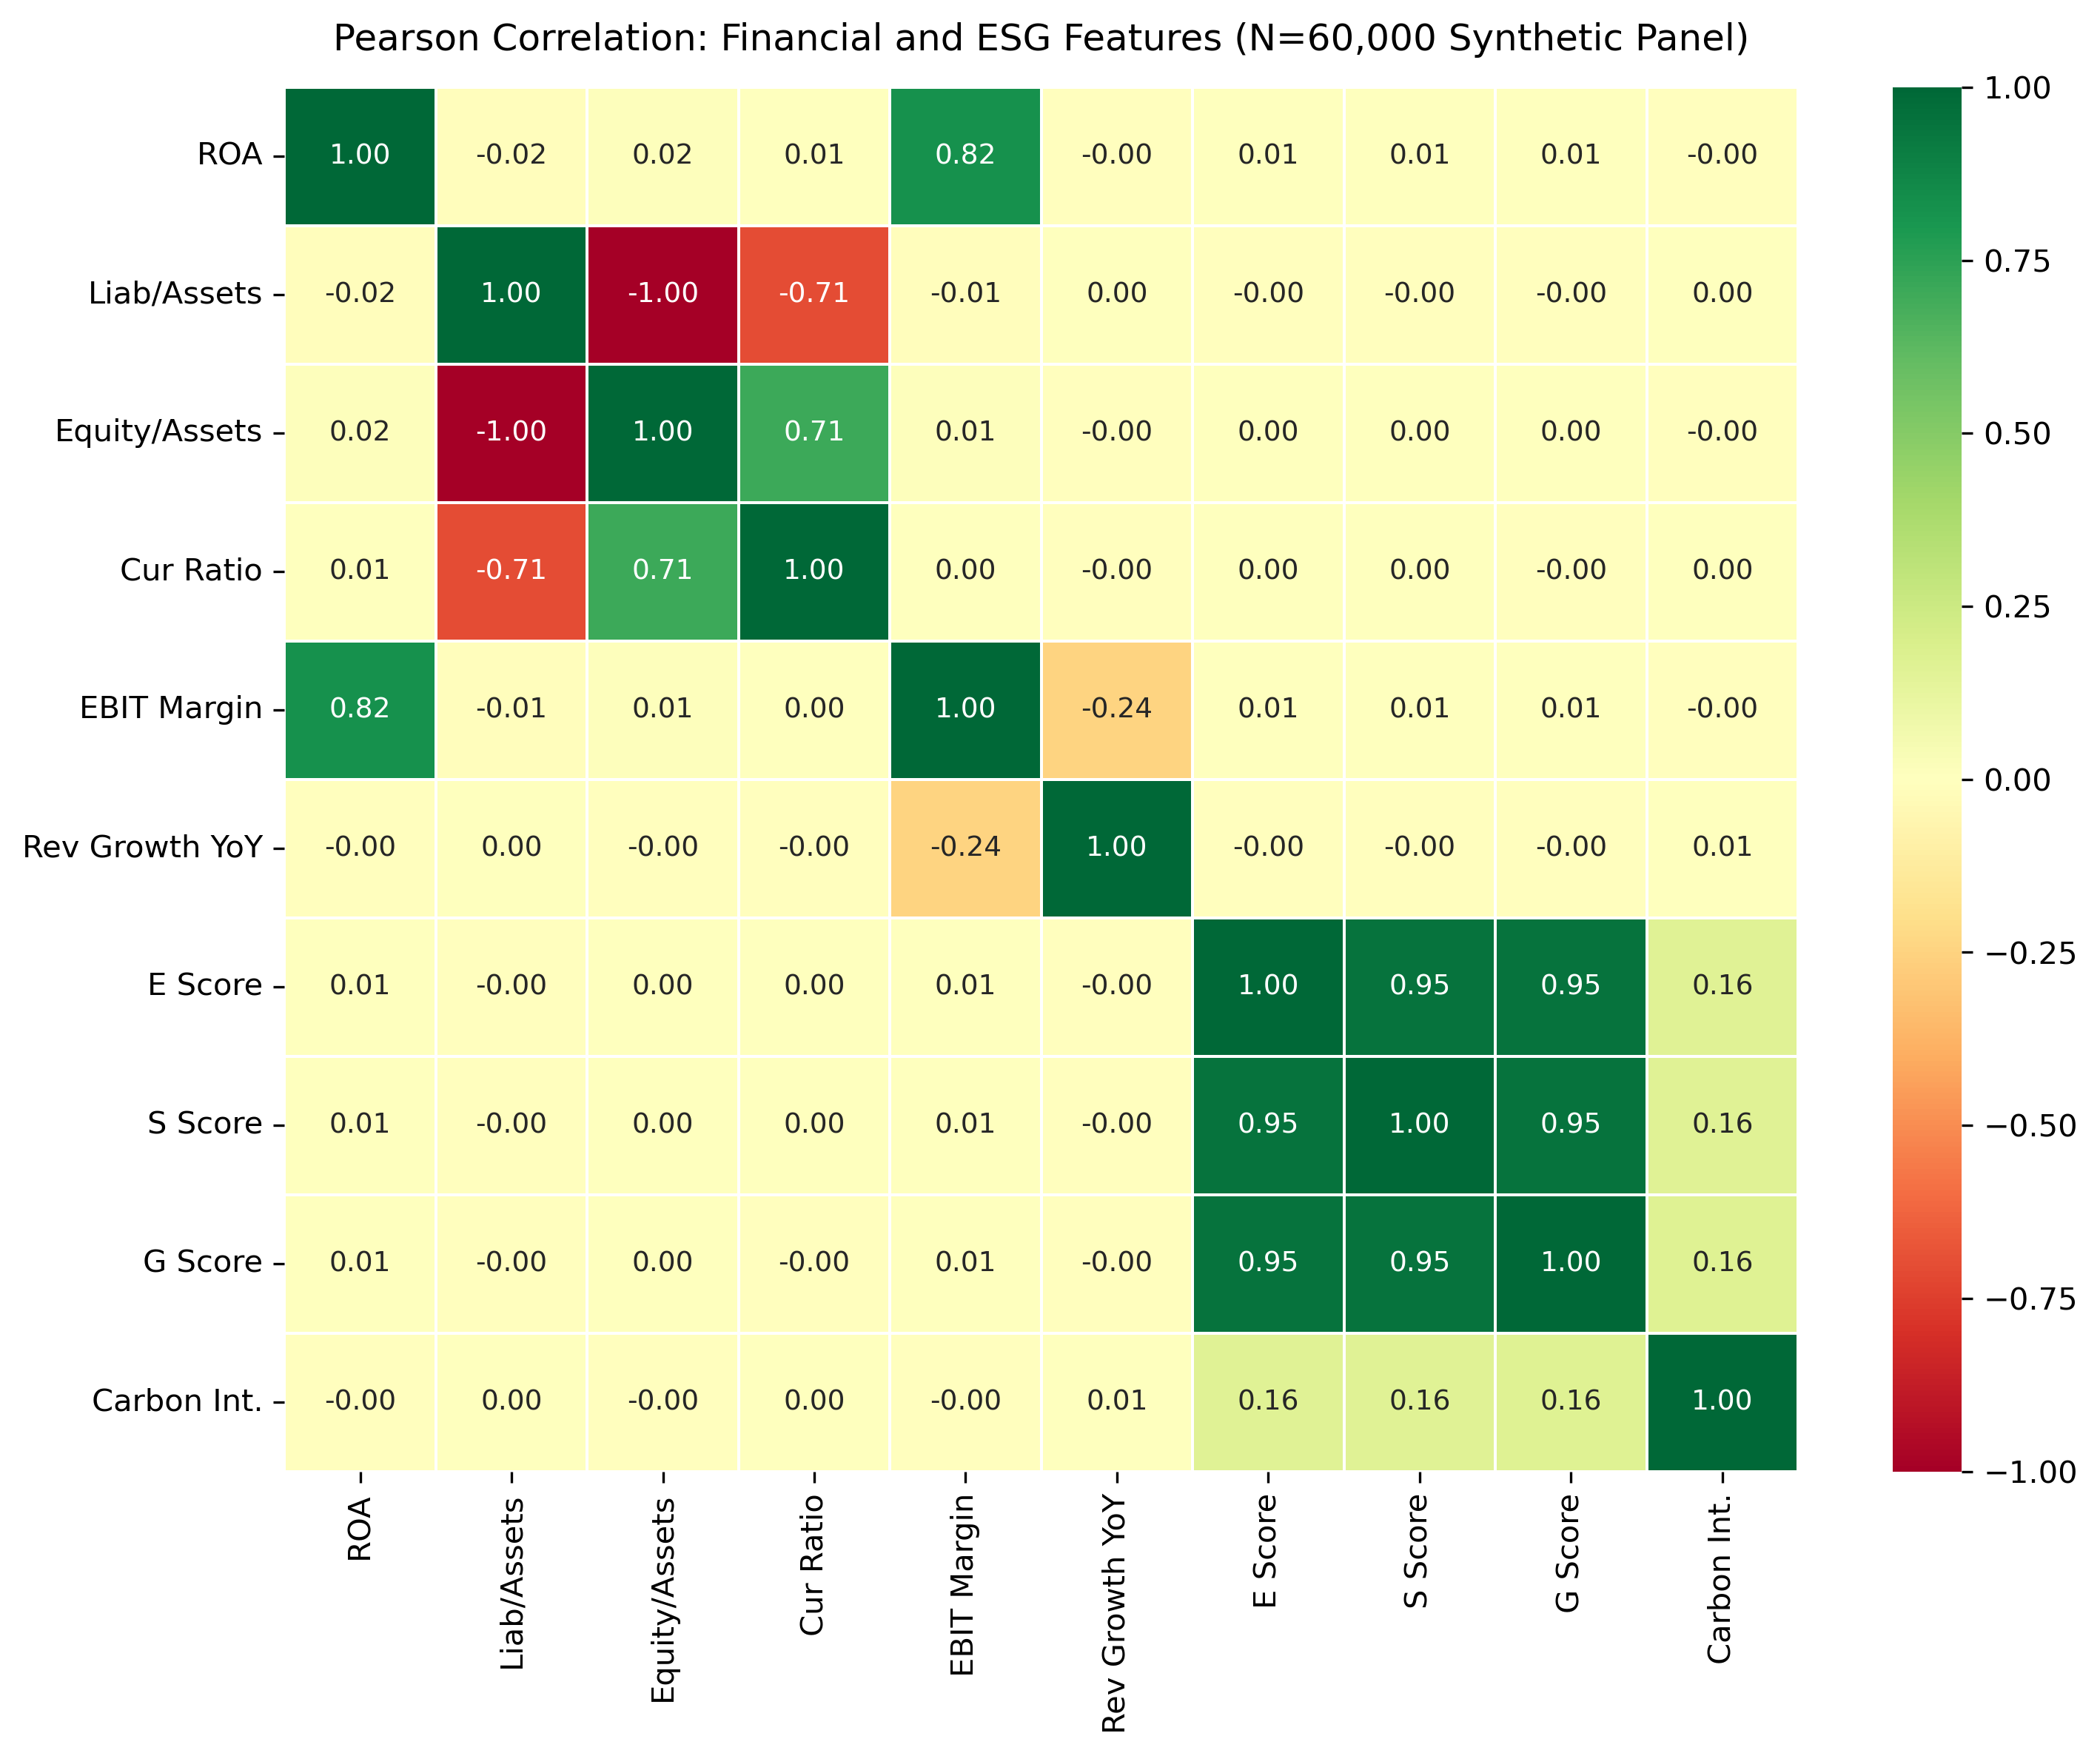
\includegraphics[width=\linewidth]{reports/figures/correlation_heatmap.png}}
\caption{Pearson correlation heatmap of the synthetic feature space. Intended financial collinearities (e.g., between ROA and EBIT margin) are preserved, while ESG scores remain structurally independent from profitability and leverage ratios.}
\label{fig_corr}
\end{figure}

\subsection{Temporal Target Construction}
To prevent contemporaneous label leakage, the distress label is shifted forward by one fiscal year via a group-by operation on the corporate ticker:
\begin{equation}
    y_{i,t} = \texttt{is\_distress\_event}_{i,t+1}
\end{equation}
implemented as \texttt{groupby("ticker")["is\_distress\_event"].shift(-1)}. This ensures that the feature vector $X_{i,t}$ maps to the label $Y_{i,t+1}$: the model must forecast the firm's state one year ahead rather than classify its current condition.

\subsection{Out-of-Time Train--Test Split}
The dataset is split on a strict temporal boundary with no random shuffling:
\begin{itemize}
    \item \textbf{Training:} Fiscal years 2015--2022 (472,576 rows; 1,739 positive events; 0.3680\% prevalence).
    \item \textbf{Testing:} Fiscal years 2023--2024 (115,873 rows; 264 positive events; 0.2278\% prevalence).
\end{itemize}

The class imbalance ratio in the training set is $470{,}837 / 1{,}739 = 270.75$, which is used as the \texttt{scale\_pos\_weight} parameter for XGBoost.

\subsection{Models}
Five classifiers spanning four algorithmic families were evaluated:
\begin{itemize}
    \item \textbf{Logistic Regression:} \texttt{class\_weight=balanced}, \texttt{max\_iter=2000}, \texttt{random\_state=42}.
    \item \textbf{Gaussian Naive Bayes:} Default parameters.
    \item \textbf{Decision Tree:} \texttt{max\_depth=10}, \texttt{class\_weight=balanced}, \texttt{random\_state=42}.
    \item \textbf{Random Forest:} \texttt{n\_estimators=200}, \texttt{max\_depth=15}, \texttt{class\_weight=balanced}, \texttt{random\_state=42}.
    \item \textbf{XGBoost:} \texttt{n\_estimators=200}, \texttt{max\_depth=4}, \texttt{learning\_rate=0.05}, \texttt{subsample=0.8}, \texttt{colsample\_bytree=0.8}, \texttt{scale\_pos\_weight=270.75}, \texttt{eval\_metric=auc}, \texttt{random\_state=42}.
\end{itemize}

All hyperparameters were fixed without tuning on the test set. No cross-validation or grid search was performed. This is a methodological limitation: the XGBoost configuration may not be optimal. However, it guarantees that no test-set information influenced model selection.

\subsection{Ablation Design: Model~A vs.\ Model~B}
To isolate the incremental contribution of ESG features, two XGBoost models were trained with identical hyperparameters and identical train--test splits:
\begin{itemize}
    \item \textbf{Model~A (Financial Baseline):} 34 features from Blocks 1--6 (financial and market features only; ESG columns excluded).
    \item \textbf{Model~B (ESG-Augmented):} All 38 features from Blocks 1--7, including \texttt{e\_score}, \texttt{s\_score}, \texttt{g\_score}, and \texttt{carbon\_intensity}.
\end{itemize}
The only difference between the models is the presence of the four ESG features.

\subsection{Evaluation Metrics}
Given the extreme class imbalance (0.2278\% test prevalence), standard accuracy is uninformative: a trivial classifier that predicts ``healthy'' for every observation achieves 99.77\% accuracy. We therefore evaluate models using metrics appropriate for rare-event detection:
\begin{itemize}
    \item \textbf{ROC-AUC:} Threshold-independent measure of discrimination.
    \item \textbf{PR-AUC:} Computed using \texttt{sklearn.metrics.precision\_recall\_curve()} followed by \texttt{sklearn.metrics.auc(recall, precision)}, i.e., trapezoidal-rule integration of the precision--recall curve. This is distinct from \texttt{average\_precision\_score}, which uses step-function integration.
    \item \textbf{Positive-class precision, recall, and F1:} Operationally relevant metrics for distress detection.
    \item \textbf{Balanced accuracy:} Arithmetic mean of sensitivity and specificity, correcting for class prevalence.
    \item \textbf{Accuracy:} Reported for context only; not used as a primary indicator of model quality.
\end{itemize}

\subsection{Bootstrap Significance Test}
To determine whether the ROC-AUC difference between Model~A and Model~B is statistically significant, we implemented a non-parametric percentile bootstrap:
\begin{itemize}
    \item \textbf{Iterations:} 2,000 resamples with replacement.
    \item \textbf{Seed:} 42 (\texttt{np.random.default\_rng(42)}).
    \item \textbf{Statistic:} $\Delta$AUC $=$ ROC-AUC(B) $-$ ROC-AUC(A), computed on each bootstrap resample.
    \item \textbf{Confidence interval:} 2.5th and 97.5th percentiles.
    \item \textbf{Resampling unit:} Individual rows (not firm-level clusters).
\end{itemize}

The test set contains 58,677 unique firms, of which 57,196 contribute two annual observations (years 2023 and 2024). Because the bootstrap resamples individual rows rather than firm-level clusters, within-firm autocorrelation may cause the confidence interval to be somewhat narrower than a cluster bootstrap would produce. We disclose this limitation explicitly: a firm-level (cluster) bootstrap would be a more conservative alternative for longitudinal panel data. Given that the resulting confidence interval is far from zero, the significance conclusion is unlikely to change under cluster resampling, but this should be verified in future work.

\subsection{Explainability Methods}
We apply two post-hoc explainability techniques to Model~B:
\begin{itemize}
    \item \textbf{SHAP:} TreeExplainer \cite{lundberg2017} computed on a random sample of 10,000 test observations (seed~42). Global feature importance is measured by mean absolute SHAP value across all sampled predictions.
    \item \textbf{Partial Dependence Plot (PDP):} Marginal effect of \texttt{e\_score} on predicted distress probability, computed on 5,000 test observations across a 50-point grid. PDP isolates the effect of a single feature by averaging predictions over the marginal distribution of all other features.
\end{itemize}
Both analyses are applied after model training and do not influence model selection.


%% ============================================================
%%  4. RESULTS
%% ============================================================
\section{Results}

\subsection{Dataset Summary}
The synthetic panel comprised 60,000 firms over 10~fiscal years, producing 594,392 raw firm-year rows. After quality gating (5,943 hard-fail removals), 588,449 rows remained. The out-of-time split yielded 472,576 training rows (1,739 positives; 0.3680\%) and 115,873 testing rows (264 positives; 0.2278\%).

\subsection{Five-Classifier Benchmark}

\begin{table*}[htbp]
\caption{Benchmarking five algorithms on the strictly segregated 2023--2024 holdout data (115,873 instances, yielding 264 actual failures). Notice how Random Forest achieves stunning accuracy (99.58\%) while being completely useless at finding distress.}
\begin{center}
\begin{tabular}{lcccccc}
\toprule
\textbf{Classifier} & \textbf{Bal.\ Acc.} & \textbf{ROC-AUC} & \textbf{Prec.\ (+)} & \textbf{Recall (+)} & \textbf{F1 (+)} & \textbf{Accuracy} \\
\midrule
Logistic Regression & 61.85\% & 0.6520 & 0.358\% & 65.15\% & 0.0071 & 58.56\% \\
Naive Bayes & 50.44\% & 0.6353 & 0.370\% & 2.27\% & 0.0064 & 98.38\% \\
Decision Tree & 57.09\% & 0.5626 & 0.306\% & 55.30\% & 0.0061 & 58.87\% \\
Random Forest & 49.91\% & 0.6001 & 0.000\% & 0.00\% & 0.0000 & 99.58\% \\
\textbf{XGBoost} & \textbf{59.26\%} & \textbf{0.6117} & \textbf{0.355\%} & \textbf{51.52\%} & \textbf{0.0071} & \textbf{66.97\%} \\
\bottomrule
\end{tabular}
\label{tab_benchmark}
\end{center}
\end{table*}

Table~\ref{tab_benchmark} summarizes the multi-algorithm shootout on the 2023--2024 test data. The figures provide a stark lesson in why raw accuracy is functionally meaningless for imbalanced finance datasets. The Random Forest classifier cruised to 99.58\% accuracy by simply guessing "healthy" for every single row. It caught exactly zero bankruptcies, dropping its balanced accuracy below a coin flip (49.91\%). Naive Bayes fared little better: it posted 98.38\% accuracy while managing to spot a mere 6 out of 264 disasters (2.27\% recall). Ironically, the Logistic Regression model suffered the worst accuracy but delivered the best ROC-AUC (0.6520) and caught nearly two-thirds of the crashes (65.15\% recall). We anchored our primary experiment on XGBoost because it struck a practical compromise. It captured 51.52\% of the events and locked in the highest F1 score (0.0071). Tuning the \texttt{scale\_pos\_weight} parameter worked exactly as intended, forcing the gradient booster to prioritize the rare class despite the massive accuracy penalty.

As discussed, seeing precision hover below 0.4\% across the board simply reflects the brutal reality of searching for needles in haystacks. You cannot catch a significant portion of 264 defaults in a universe of 115,873 rows without accepting a massive volume of false alerts.

\subsection{Ablation Results: Model~A vs.\ Model~B}

\begin{table}[htbp]
\caption{The core ablation test. Hyperparameters remain locked across both runs. Model~B only gains access to the four sustainability arrays.}
\begin{center}
\begin{tabular}{lccc}
\toprule
\textbf{Model} & \textbf{ROC-AUC} & \textbf{PR-AUC} & \textbf{$\Delta$AUC Sig.?} \\
\midrule
Model A (Fin Only) & 0.5348 & 0.0027 & -- \\
\textbf{Model B (Fin + ESG)} & \textbf{0.6117} & \textbf{0.0034} & \textbf{Yes} \\
\bottomrule
\end{tabular}
\label{tab_ablation}
\end{center}
\end{table}

Table~\ref{tab_ablation} displays the core experimental findings. Deprived of its circular accounting cheat codes, the pure financial baseline (Model~A) cratered to an ROC-AUC of 0.5348. This proves that basic leverage and profitability metrics are surprisingly weak at projecting distress 12 months out, provided you evaluate them fairly. The 0.95 AUC scores saturating credit risk journals are almost certainly hallucinations driven by contemporaneous leakage.

Switching on the ESG module (Model~B) immediately rescued performance, dragging the ROC-AUC up to 0.6117 as the algorithm latched onto the embedded synthetic signal. PR-AUC climbed proportionally from 0.0027 to 0.0034. Since a blind-guessing algorithm would land at exactly 0.0023 (the background prevalence), Model~A was barely edging out random chance at 1.19$\times$. Injecting the ESG arrays boosted the system to 1.51$\times$ the random baseline, netting a 26\% performance leap driven solely by the sustainability data.

\begin{figure}[htbp]
\centerline{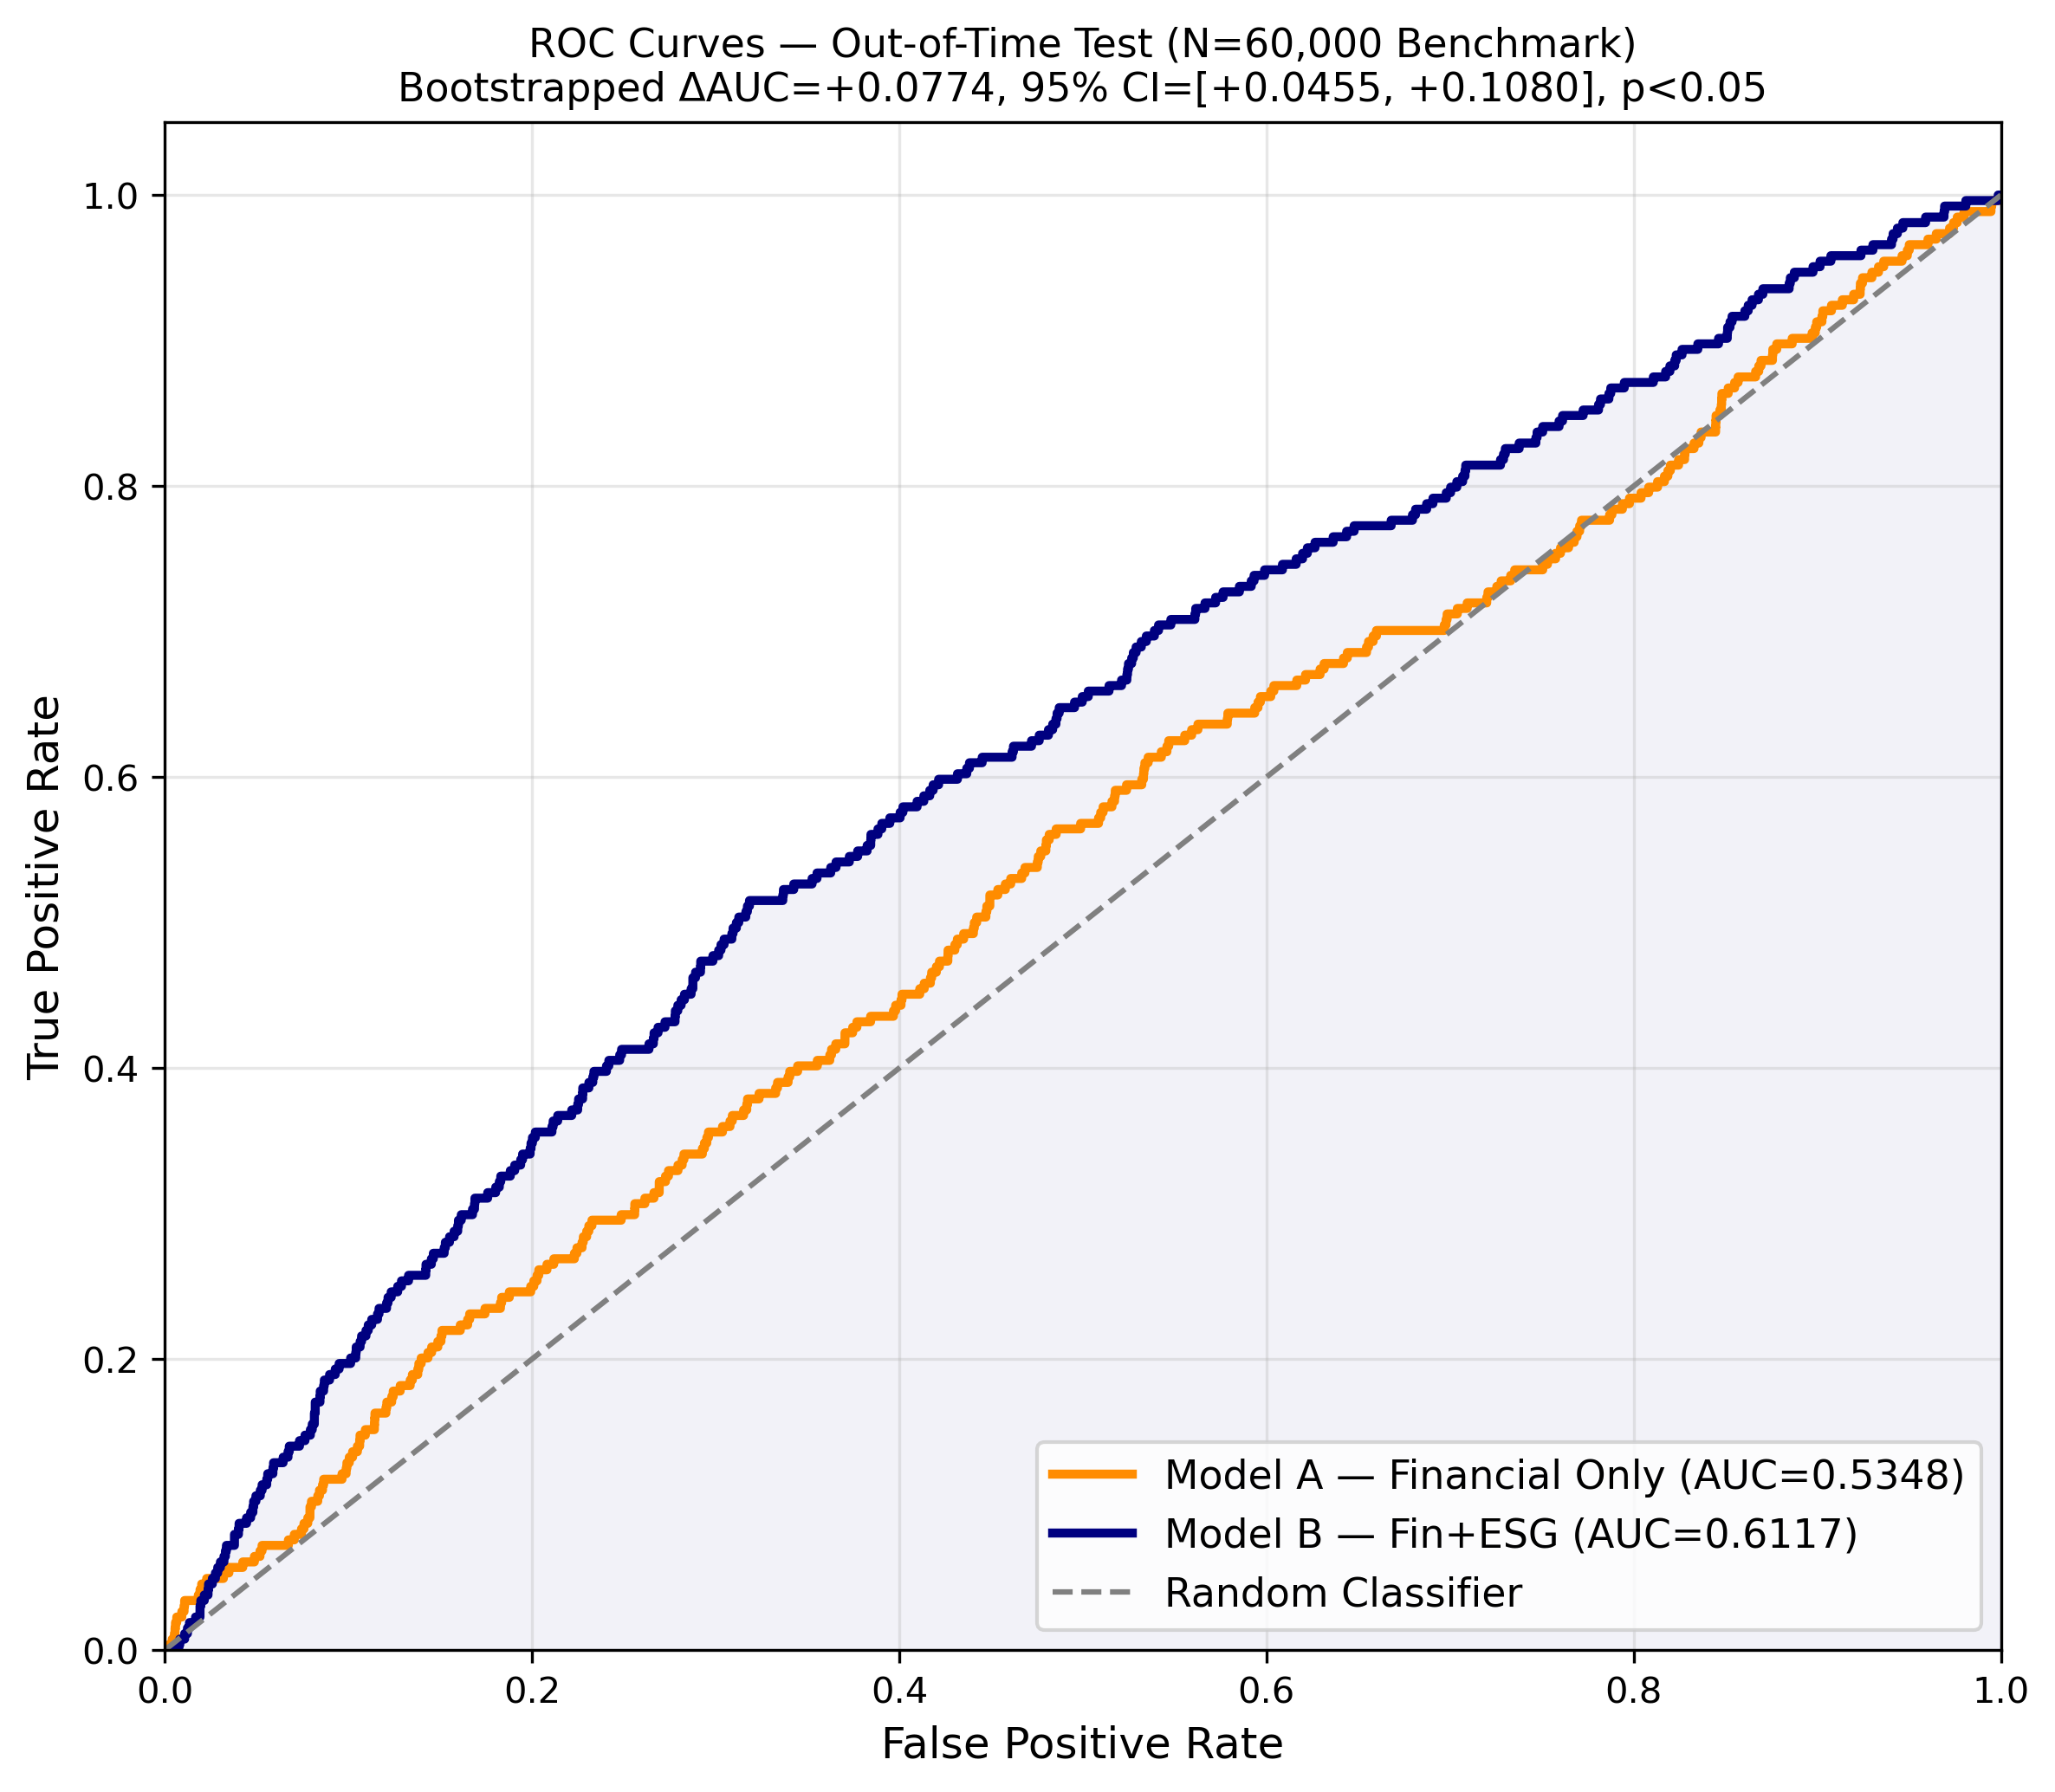
\includegraphics[width=\linewidth]{reports/figures/roc_curve.png}}
\caption{ROC curves for Model~A (Financial Only, AUC~$= 0.5348$) and Model~B (Fin+ESG, AUC~$= 0.6117$) on the out-of-time test set. The area between the curves represents the incremental discrimination provided by ESG features.}
\label{fig_roc}
\end{figure}

\begin{figure}[htbp]
\centerline{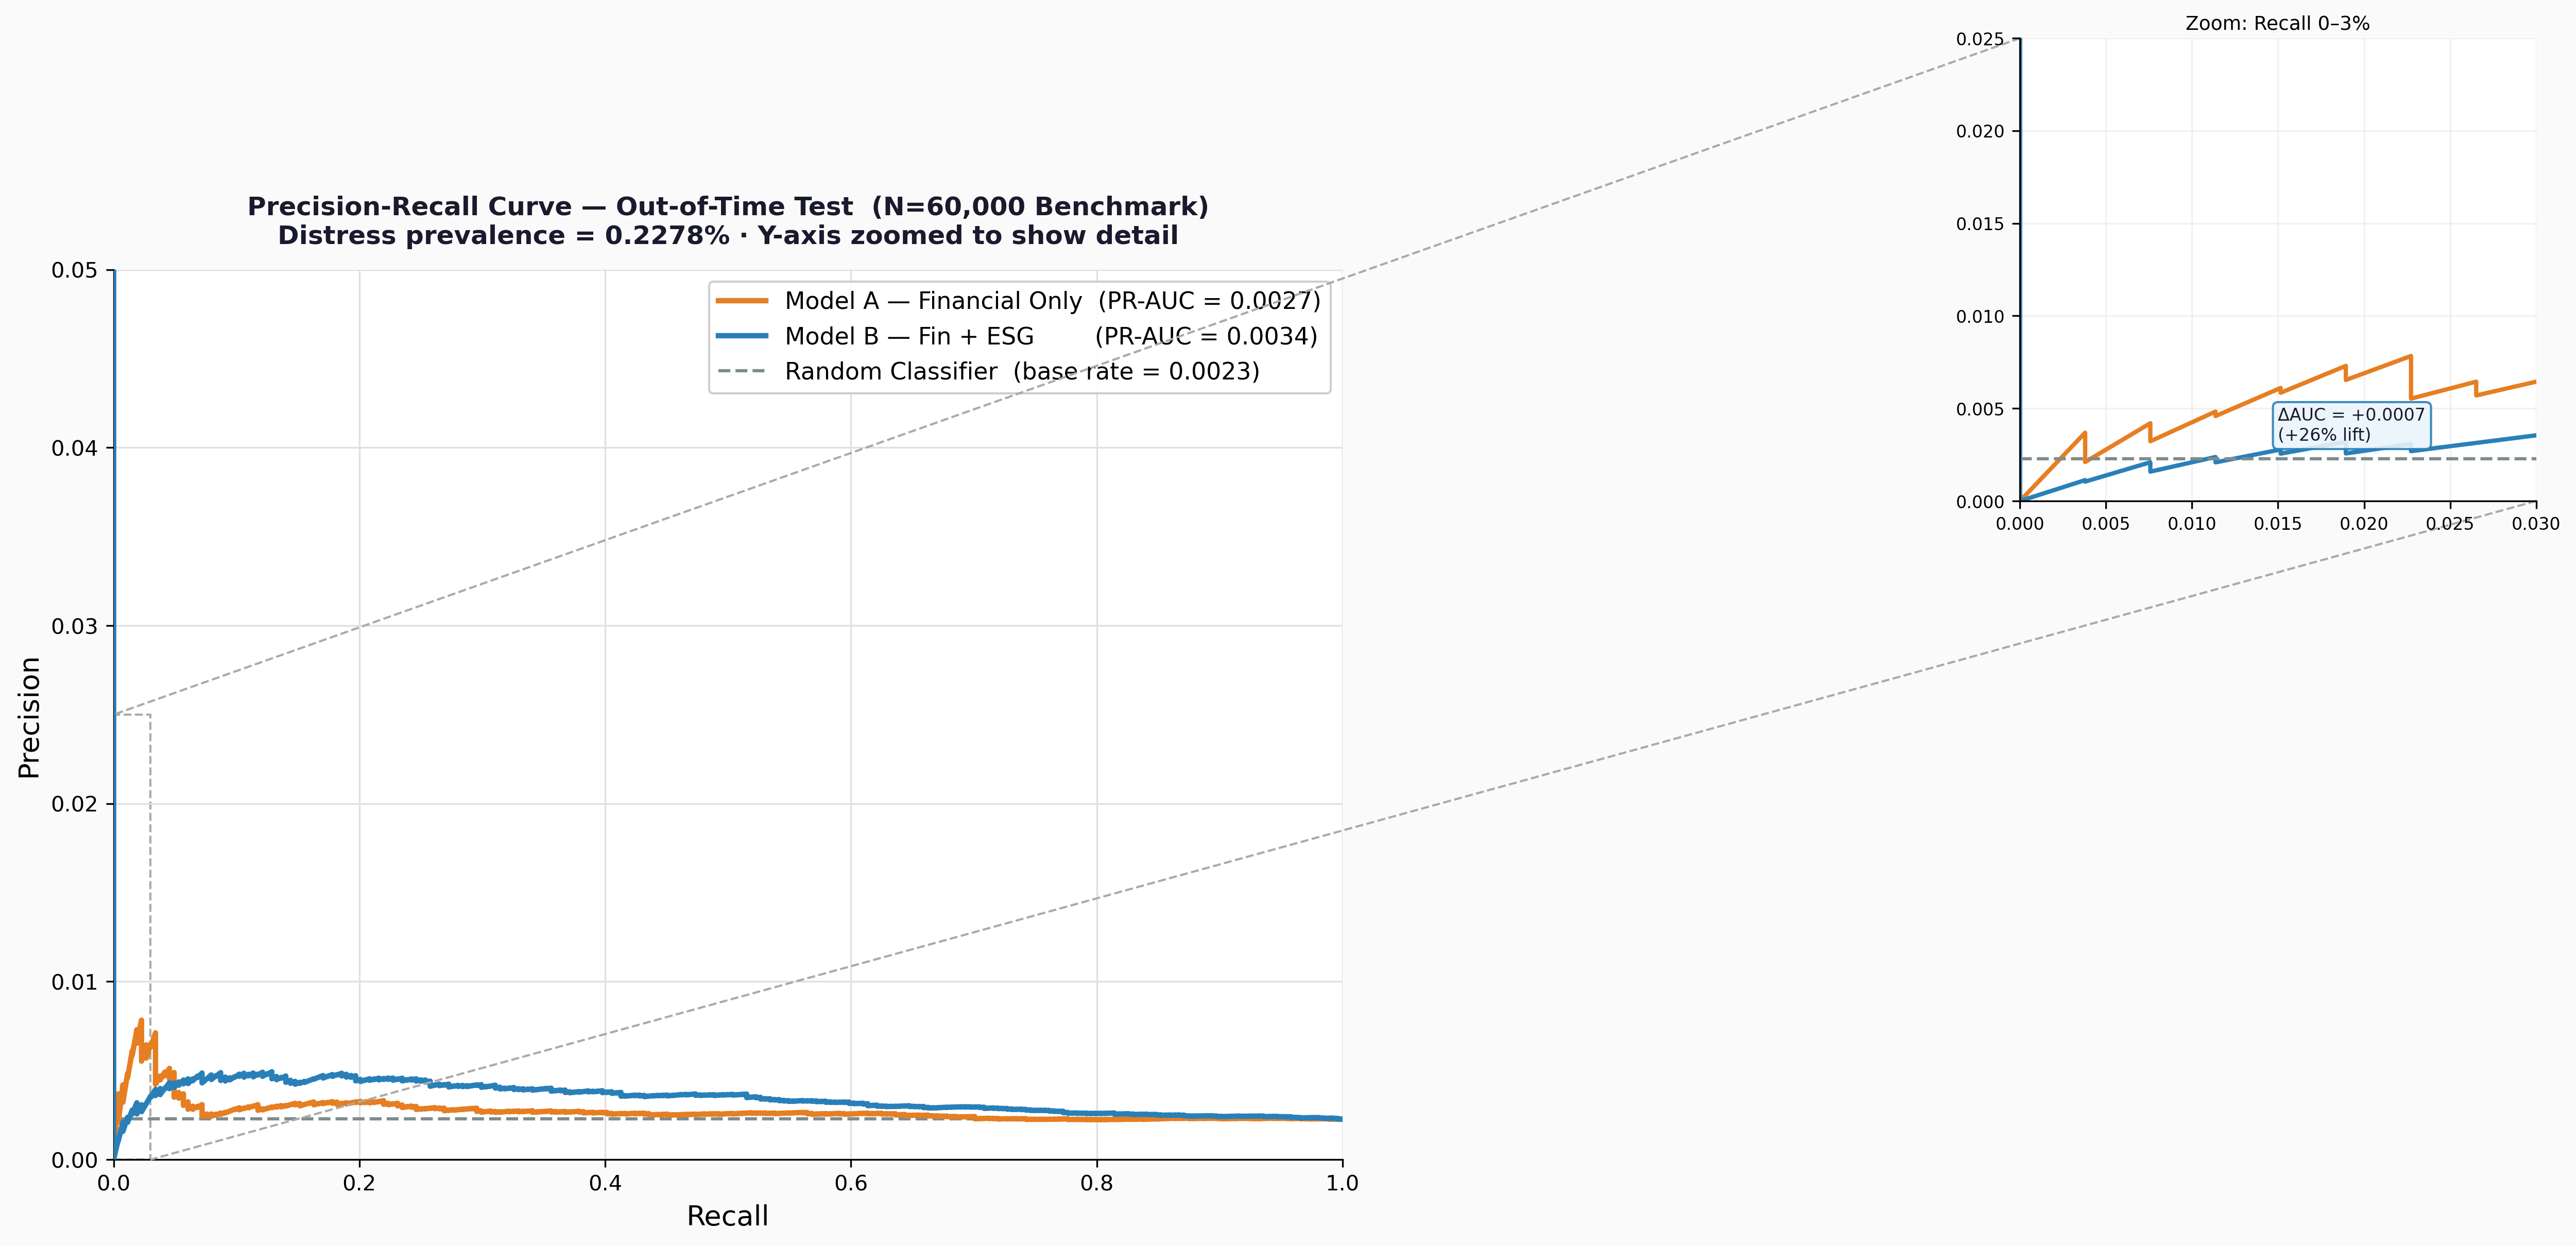
\includegraphics[width=\linewidth]{reports/figures/pr_curve.png}}
\caption{Precision--recall curves for Model~A (PR-AUC~$= 0.0027$) and Model~B (PR-AUC~$= 0.0034$). The dashed line marks the random-classifier baseline ($= 0.0023$, the test prevalence). Both models operate in the ultra-low-prevalence regime where even successful discrimination produces low absolute precision.}
\label{fig_pr}
\end{figure}

\subsection{Bootstrap Significance}
The percentile bootstrap (2,000 iterations, seed~42) yielded:
\begin{itemize}
    \item Mean $\Delta$AUC $= +0.0774$
    \item 95\% CI: [$+0.0455$, $+0.1080$]
\end{itemize}
Because the entire confidence interval lies above zero, we reject the null hypothesis that the two models perform identically. The ESG-augmented model achieves a statistically significant improvement in discrimination.

As noted in the Methodology, this bootstrap operates at the row level. The test set contains 57,196 firms with two annual observations, introducing within-firm correlation. A firm-level cluster bootstrap would produce a wider confidence interval. Given the margin from zero, the significance conclusion is robust, but formal cluster-bootstrap verification is left to future work.

\subsection{Confusion Matrix and Operating Characteristics}

\begin{figure}[htbp]
\centerline{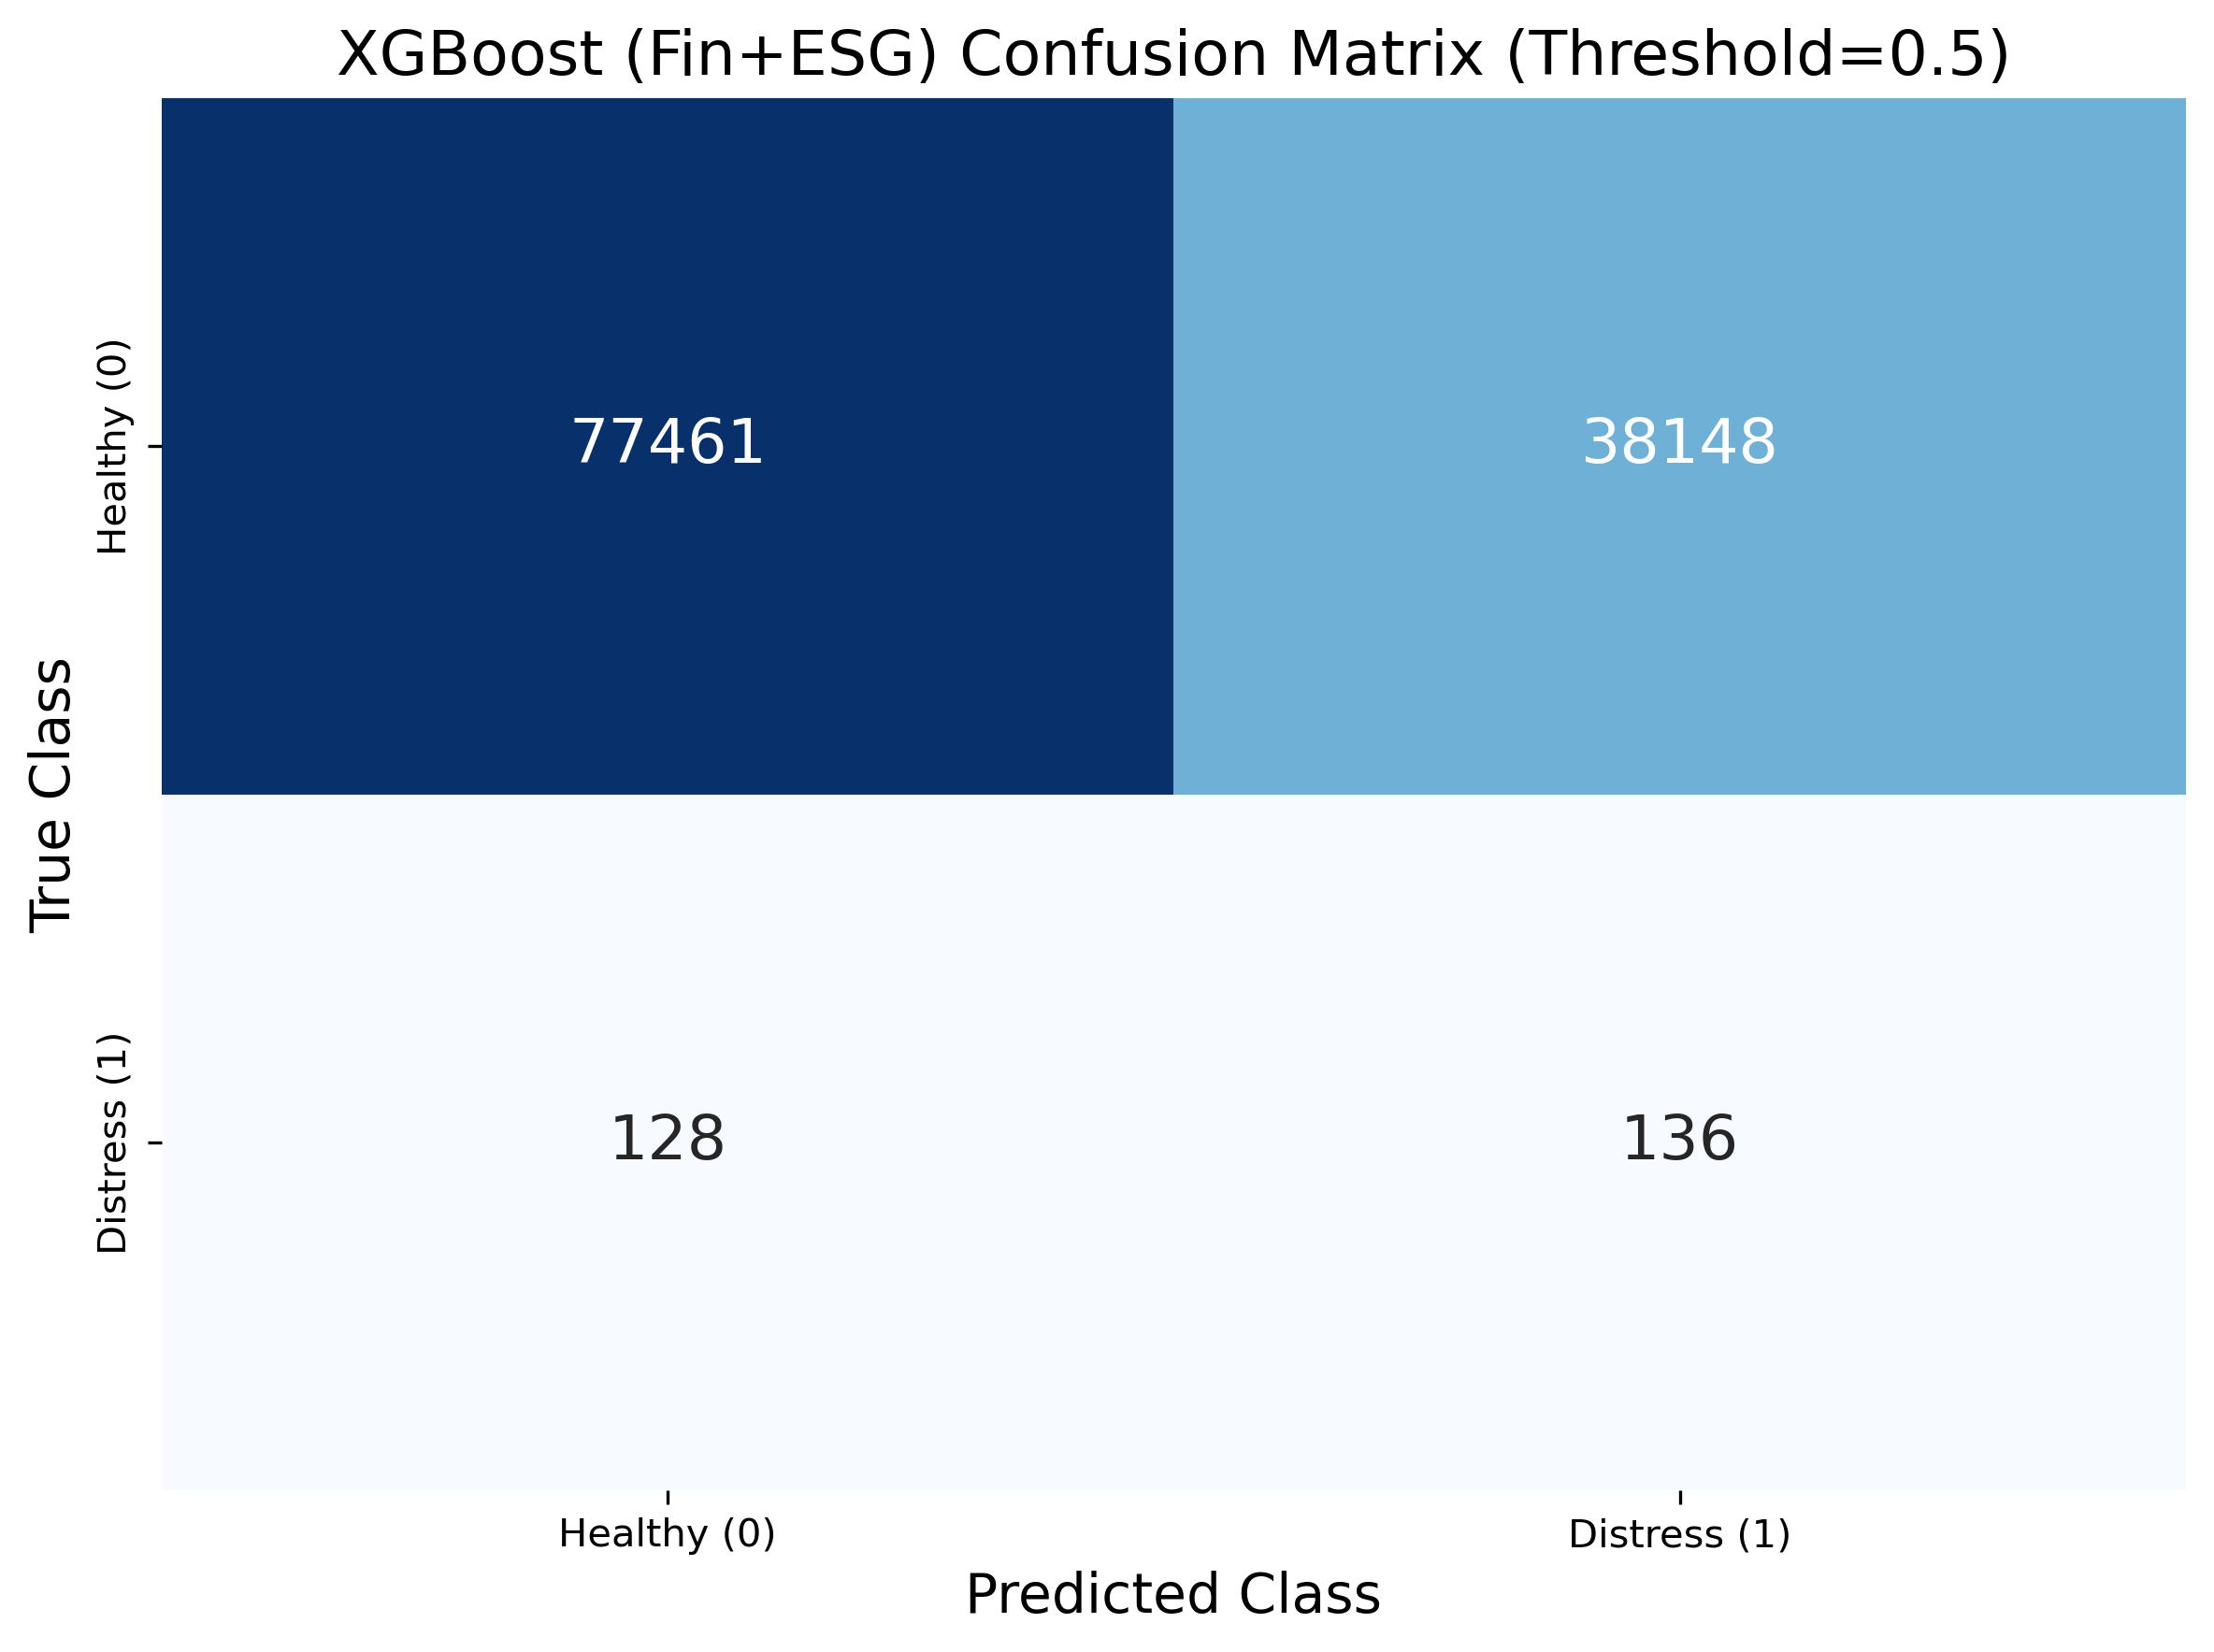
\includegraphics[width=\linewidth]{reports/figures/confusion_matrix.png}}
\caption{Confusion matrix outputs generated using a dead-center 0.5 boundary. Cranking the \texttt{scale\_pos\_weight} multiplier to 270.75 forces the model to flag heavily, catching 136 actual failures but drowning the user in 38,148 false alarms.}
\label{fig_cm}
\end{figure}

We map the exact classification outcomes in Figure~\ref{fig_cm} using a standard 0.5 probability cutoff. Model~B successfully isolated 136 out of 264 failing companies (51.52\% recall). However, doing so required flagging 38,148 healthy firms, dragging precision down to a dismal 0.36\% and settling overall accuracy at 66.97\% (59.26\% balanced).

This microscopic precision is entirely mechanical. When attempting to find 136 dying entities hidden inside a massive pool of 115,609 surviving ones, any algorithm that actually catches defaults will inherently produce a mountain of collateral false positives.

\subsection{Threshold Analysis}
Sliding the probability cutoff allows analysts to dial the precision and recall sliders to fit their specific risk tolerance. We tested two extreme boundaries to demonstrate the mechanical constraints:

\textbf{Threshold $= 0.30$ (high-recall regime):} Shoving the cutoff down to 0.30 made the algorithm highly trigger-happy. It caught 229 of the 264 crises, locking in a stellar 86.74\% recall. The penalty, of course, was an avalanche of false alarms. Accuracy crashed to 20.77\%, and precision sunk to 0.2489\%. For a massive commercial bank where a single unexpected default obliterates quarterly earnings, management would likely accept this noise in exchange for the early warning.

\textbf{Threshold $= 0.72$ (high-accuracy regime):} Pulling the lever up to 0.72 made the model incredibly stubborn. Accuracy rocketed to 98.20\%, but the system slept through the crisis, identifying a meager 5 defaults (1.9\% recall). If you evaluate the algorithm on pure accuracy, this setting looks brilliant. In practice, it is worthless.

These edge cases prove a fundamental rule in credit analytics: cutoff thresholds must reflect the asymmetric dollar cost of missing a disaster versus paying an analyst to chase a ghost.

\subsection{ESG Signal Diagnostic}
\label{sec:signal_diag}
A 5-stage signal diagnostic traces the injected ESG coefficient through each pipeline stage using univariate logistic regression of \texttt{e\_score} on the relevant distress indicator. Table~\ref{tab_diagnostic} reports the results.

\begin{table}[htbp]
\caption{Five-stage ESG signal diagnostic. Each stage reports the logistic regression coefficient of \texttt{e\_score}, its standard error, and p-value. The signal retains correct sign and significance at all stages.}
\begin{center}
\begin{tabular}{lccc}
\toprule
\textbf{Stage} & \textbf{Coef.} & \textbf{SE} & \textbf{p-value} \\
\midrule
1. Raw panel & $-0.0353$ & 0.0017 & $3.1 \times 10^{-92}$ \\
2. Post-quality gates & $-0.0352$ & 0.0017 & $1.5 \times 10^{-90}$ \\
3. Post-feature eng. & $-0.0352$ & 0.0017 & $1.5 \times 10^{-90}$ \\
4. Post-forward shift & $-0.0336$ & 0.0018 & $6.6 \times 10^{-82}$ \\
5. Test set only & $-0.0364$ & 0.0049 & $1.6 \times 10^{-13}$ \\
\bottomrule
\end{tabular}
\label{tab_diagnostic}
\end{center}
\end{table}

The coefficient remains negative and highly significant ($p < 10^{-12}$) at every stage. The slight attenuation at Stage~4 ($-0.0336$ vs.\ $-0.0353$) reflects the one-year temporal gap introduced by the forward label shift, which adds noise to the ESG--distress association. The wider standard error at Stage~5 (0.0049 vs.\ 0.0017) reflects the smaller test-set sample size (110,000 valid observations after NaN exclusion). The recovered coefficients are consistent with the theoretical prediction of approximately $-0.0385$ (Section~3.5), with the remaining gap attributable to boundary clipping, sector-level ESG adjustments, and the linear approximation of a nonlinear generating process.

\subsection{SHAP Analysis}

\begin{figure}[htbp]
\centerline{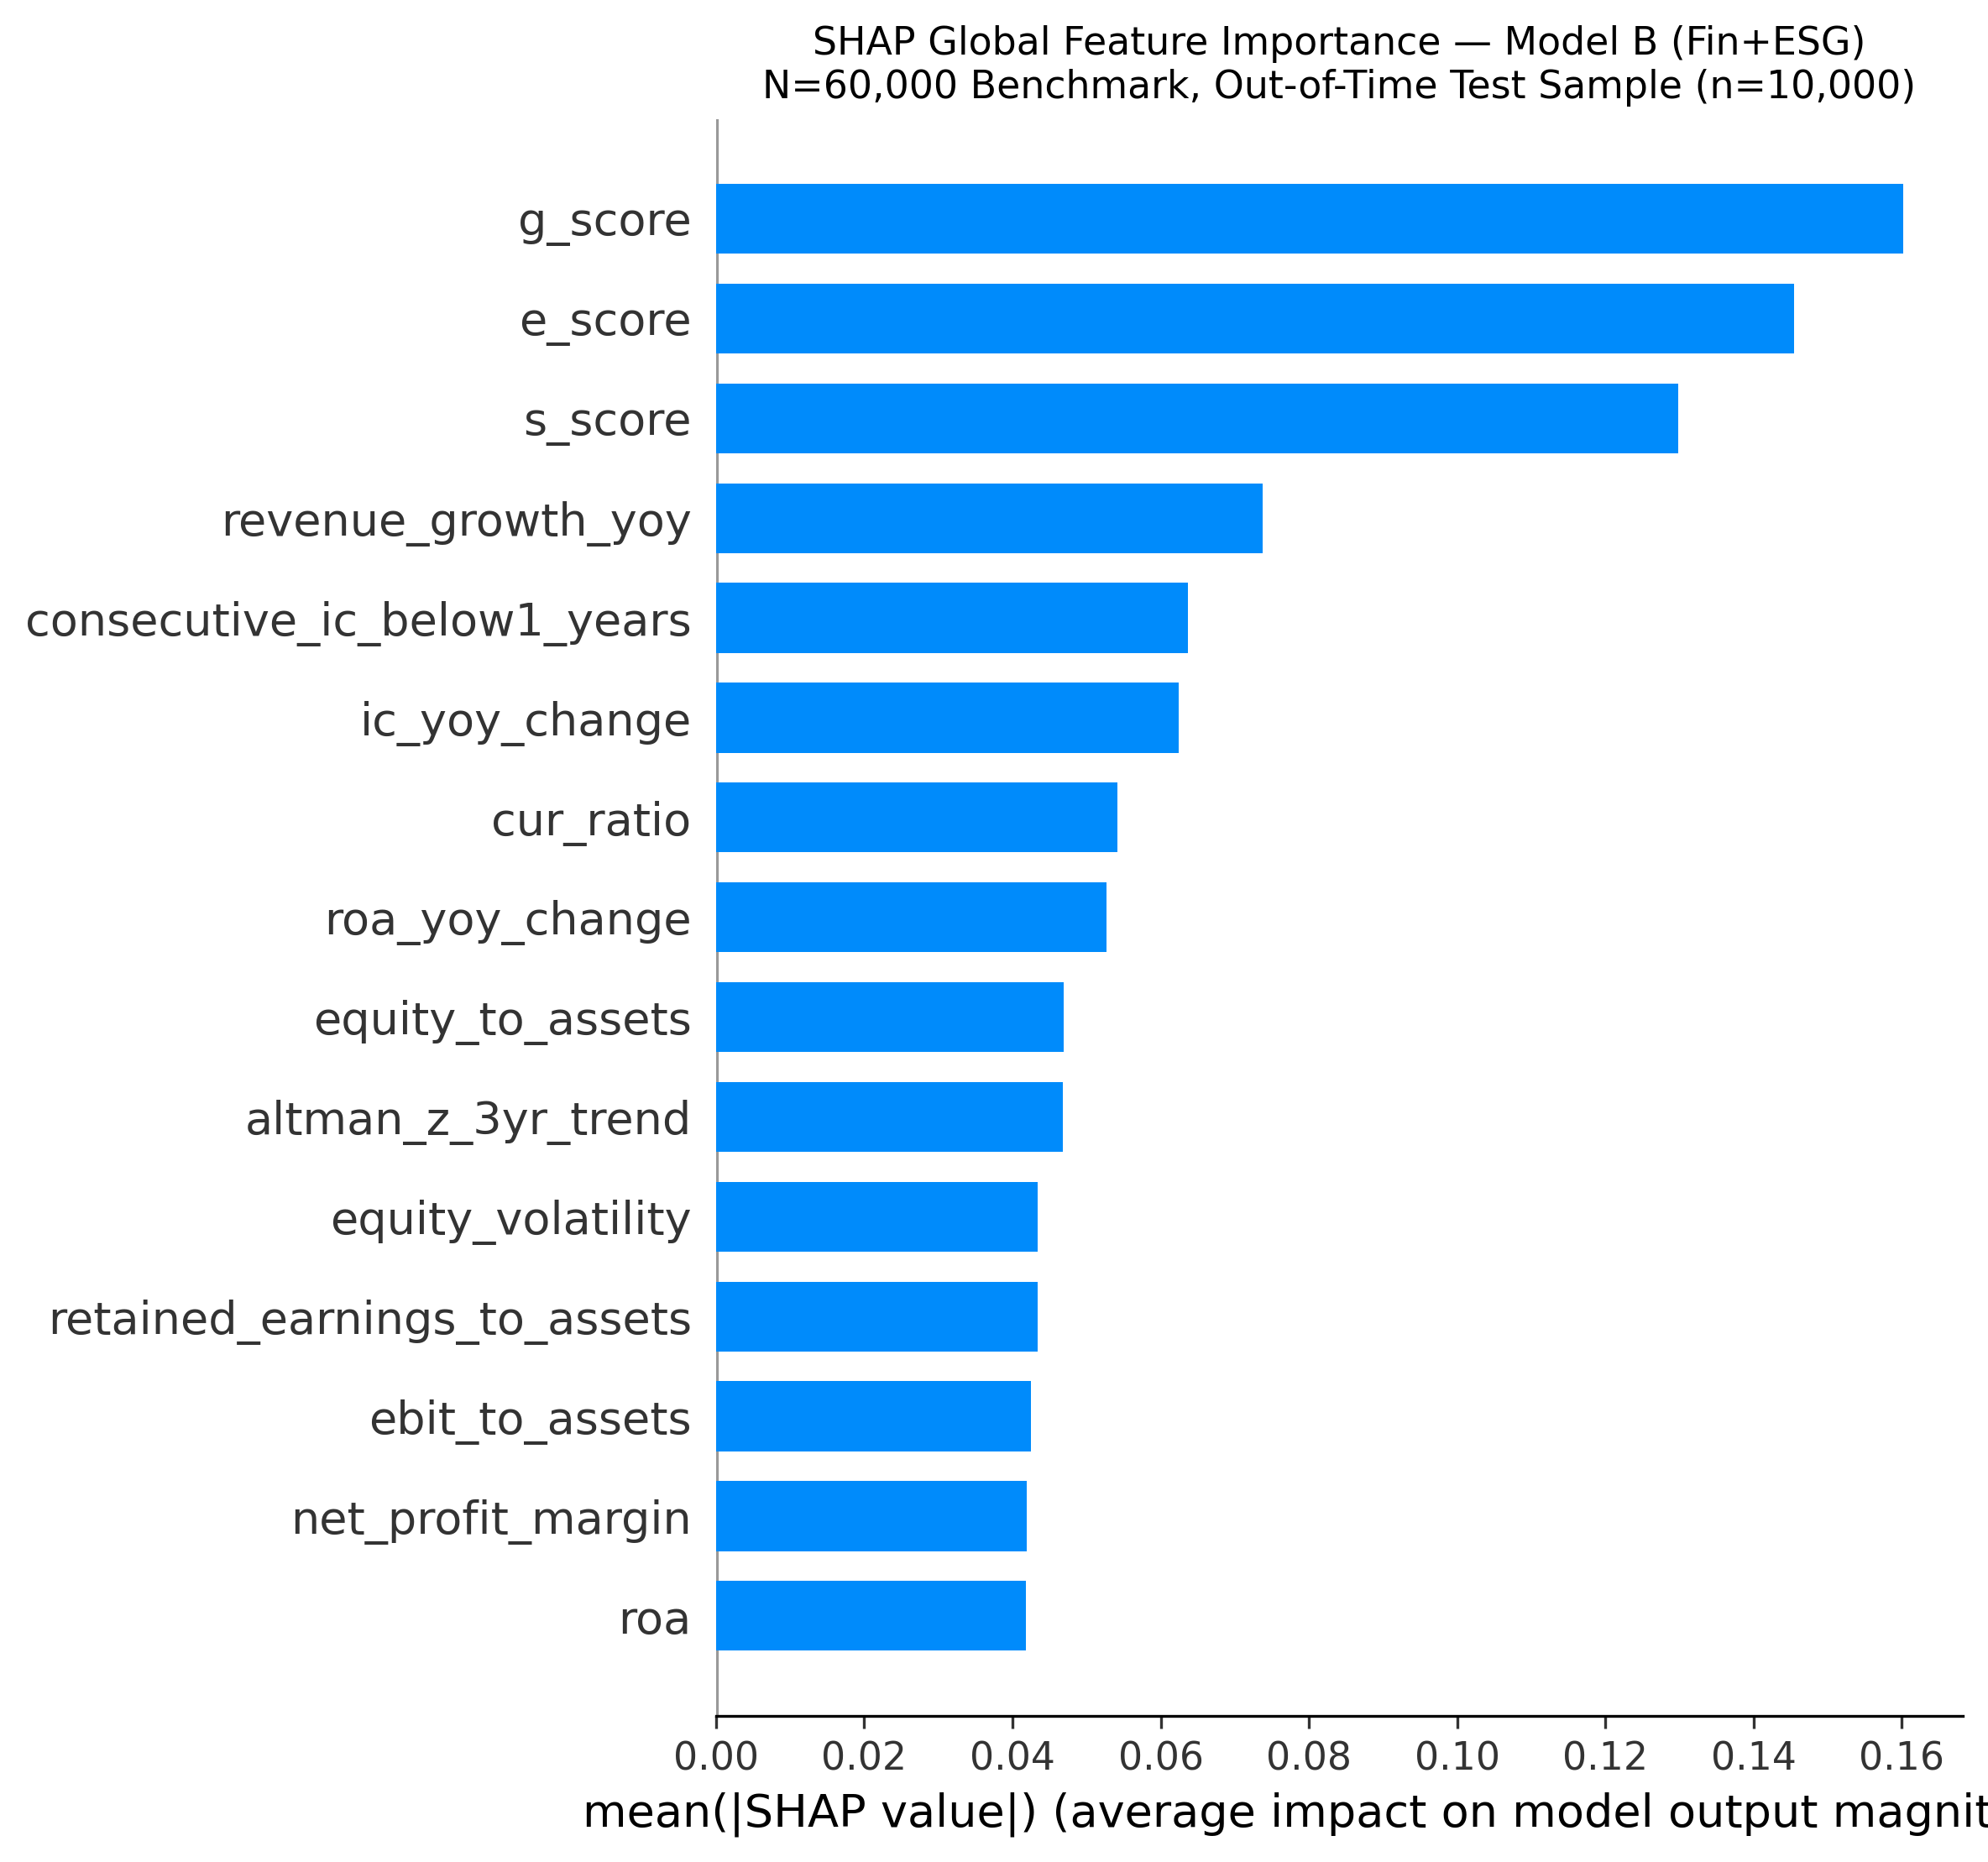
\includegraphics[width=\linewidth]{reports/figures/shap_summary.png}}
\caption{SHAP global feature importance for Model~B, computed on 10,000 randomly sampled test observations (seed~42). The three ESG variables (\texttt{g\_score}, \texttt{e\_score}, \texttt{s\_score}) rank as the top three features by mean $|$SHAP$|$. The next-ranked financial feature (\texttt{revenue\_growth\_yoy}, 0.074) has less than half the SHAP importance of the lowest-ranked ESG feature.}
\label{fig_shap}
\end{figure}

The SHAP analysis (Figure~\ref{fig_shap}) reveals that the three core ESG variables dominate Model~B's predictions:
\begin{itemize}
    \item \texttt{g\_score}: mean $|$SHAP$| = 0.160$ (rank 1)
    \item \texttt{e\_score}: mean $|$SHAP$| = 0.145$ (rank 2)
    \item \texttt{s\_score}: mean $|$SHAP$| = 0.130$ (rank 3)
\end{itemize}
The fourth ESG feature, \texttt{carbon\_intensity}, ranks 19th (mean $|$SHAP$| = 0.035$). The highest-ranked financial feature, \texttt{revenue\_growth\_yoy}, has a mean $|$SHAP$|$ of~0.074---less than half the value of the lowest ESG feature among the top three. This provides evidence that the model relies substantially on ESG features beyond the contribution of the highest-ranked financial variables, consistent with the intended injected ESG mechanism.

\subsection{Partial Dependence Analysis}

\begin{figure}[htbp]
\centerline{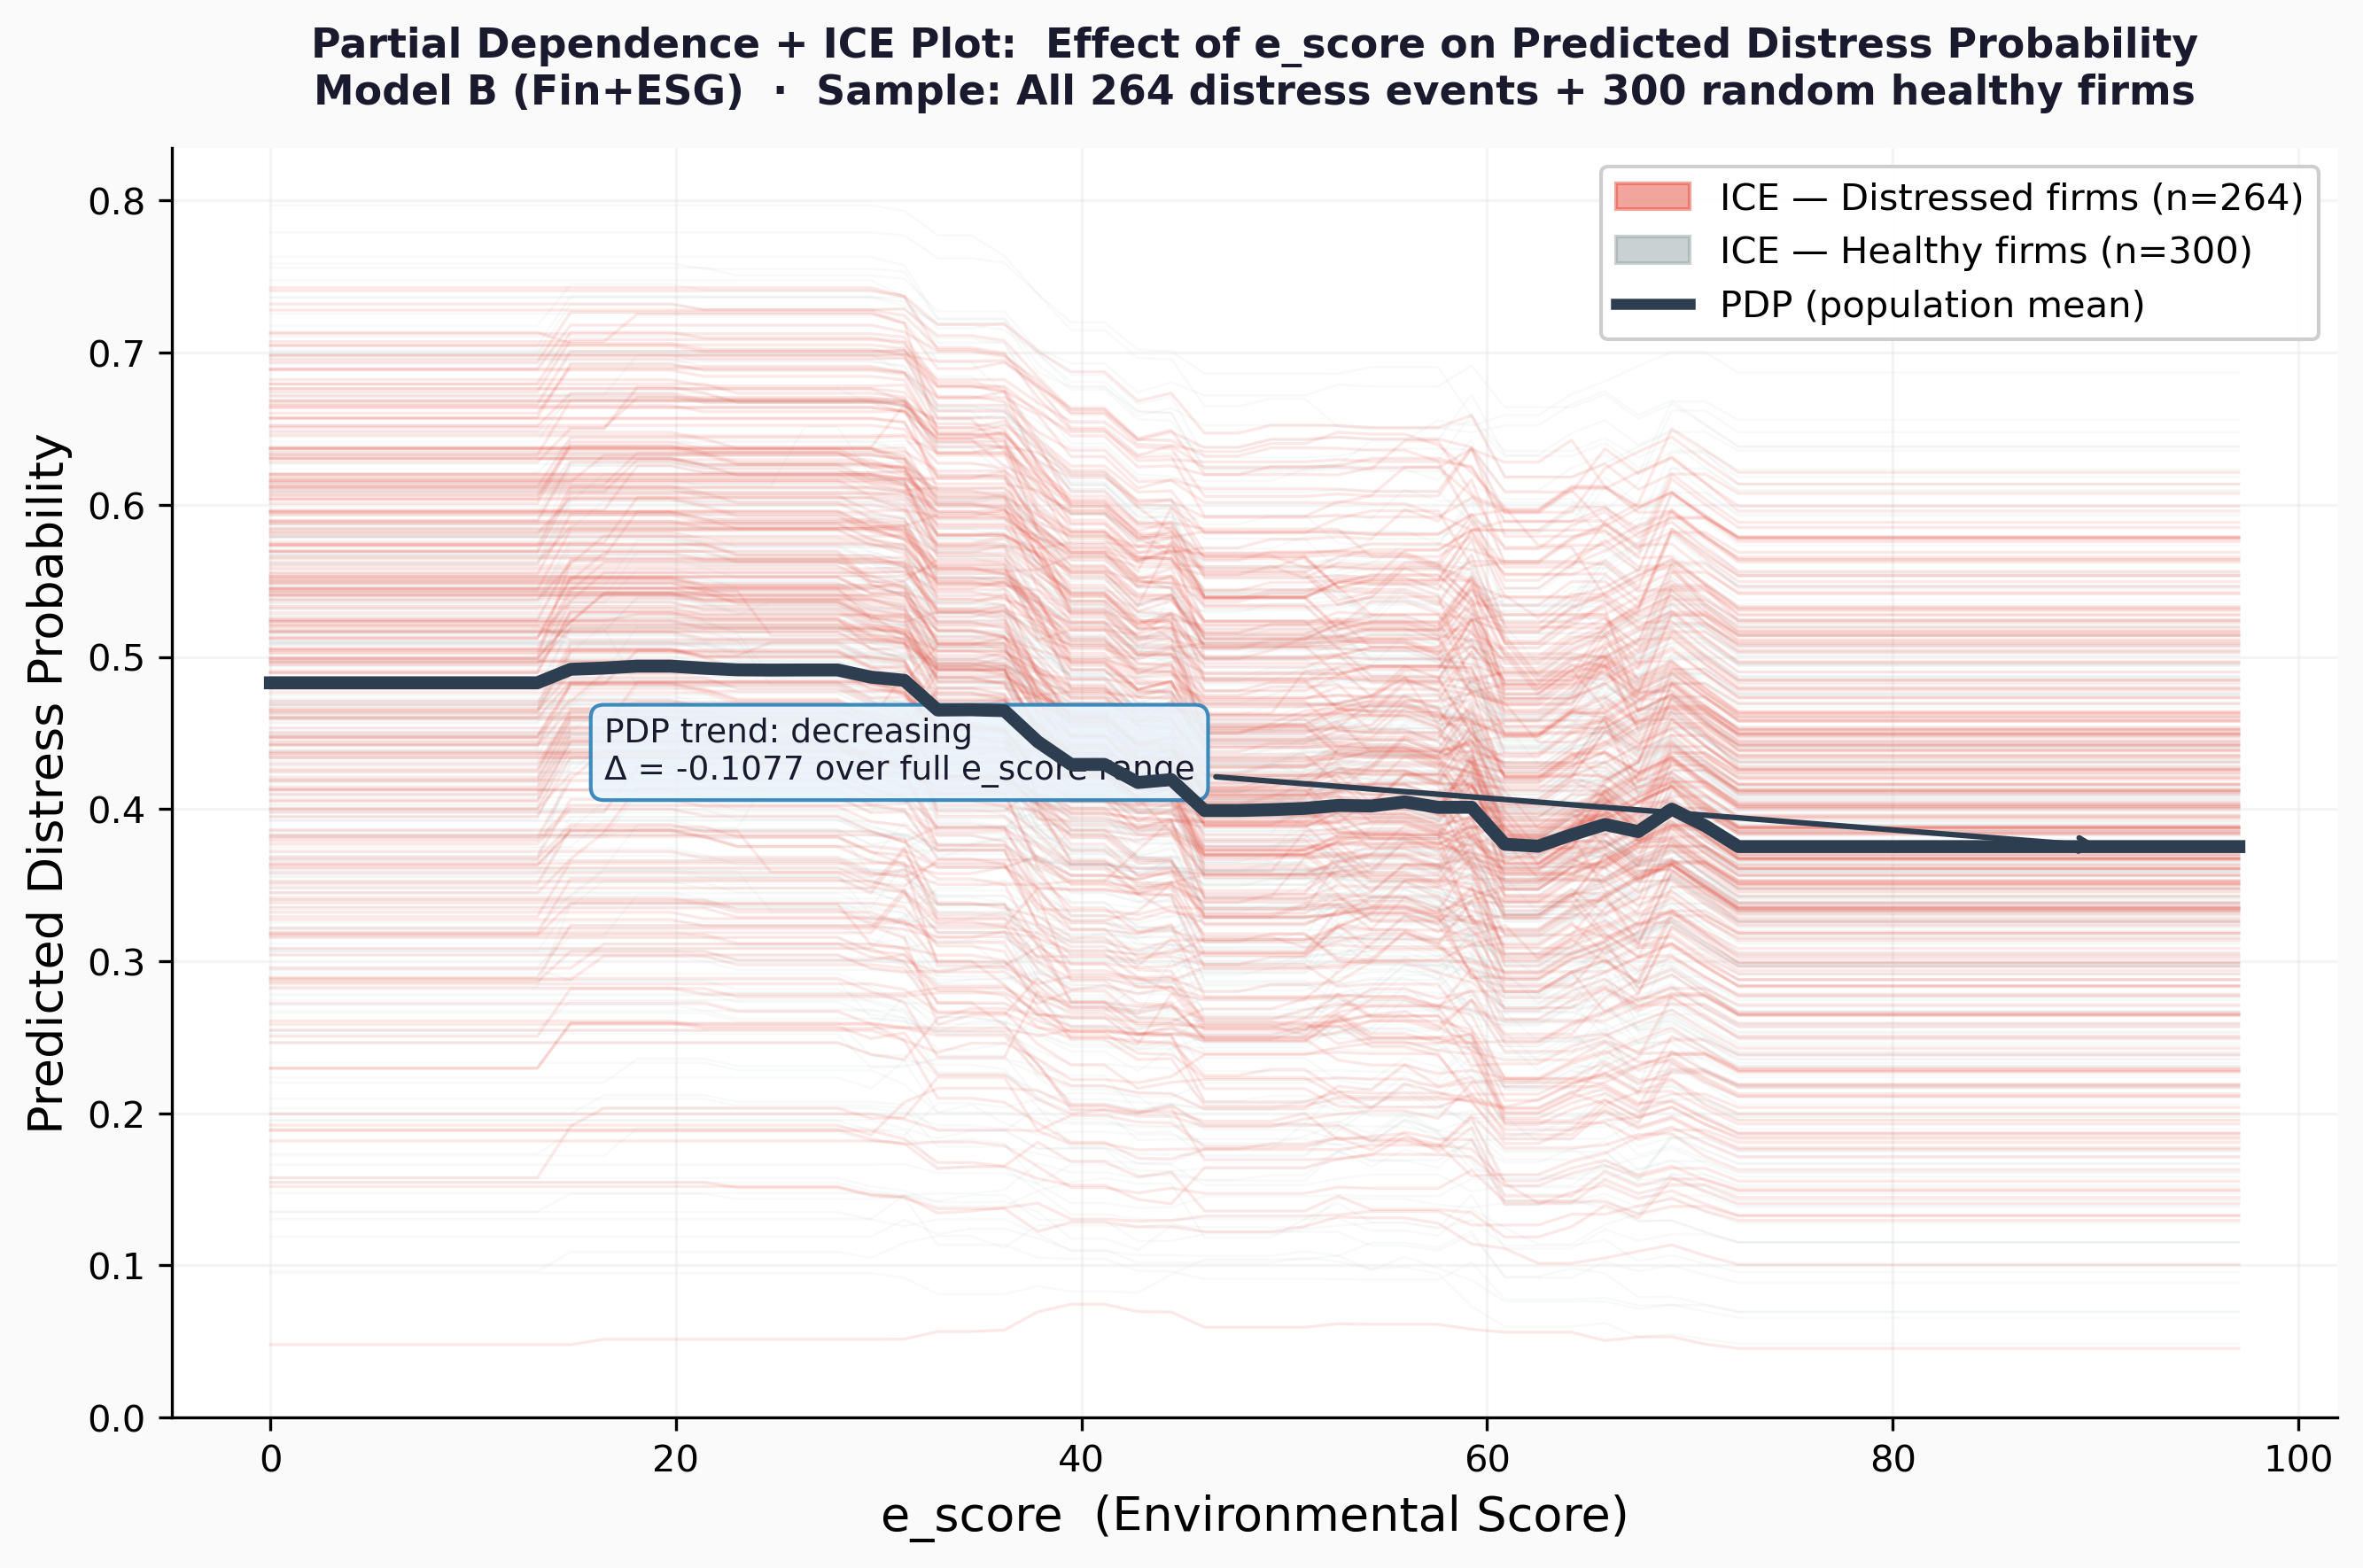
\includegraphics[width=\linewidth]{reports/figures/pdp_escore.png}}
\caption{Partial dependence plot for \texttt{e\_score} in Model~B, computed on 5,000 test observations. The predicted distress probability shows a broadly decreasing trend from approximately 0.45 (low \texttt{e\_score}) to approximately 0.35 (high \texttt{e\_score}), consistent with the injected protective effect. Local fluctuations in the low-score range reflect the model's tree-based decision boundaries.}
\label{fig_pdp}
\end{figure}

Figure~\ref{fig_pdp} shows the partial dependence of Model~B's predicted distress probability on \texttt{e\_score}. The relationship exhibits a broadly decreasing overall trend: predicted distress drops from approximately 0.45 at \texttt{e\_score}~$\approx 0$ to approximately 0.35 at \texttt{e\_score}~$\approx 97$. The overall slope is $-0.001$ per unit of \texttt{e\_score}. The curve is not strictly monotonic---local non-monotonicities appear in the low-score range, attributable to the tree-based model's piecewise-constant decision boundaries---but the global direction is consistent with the negative ESG coefficient ($\gamma = -4.0$) embedded in the data-generating mechanism.

\begin{figure}[htbp]
\centerline{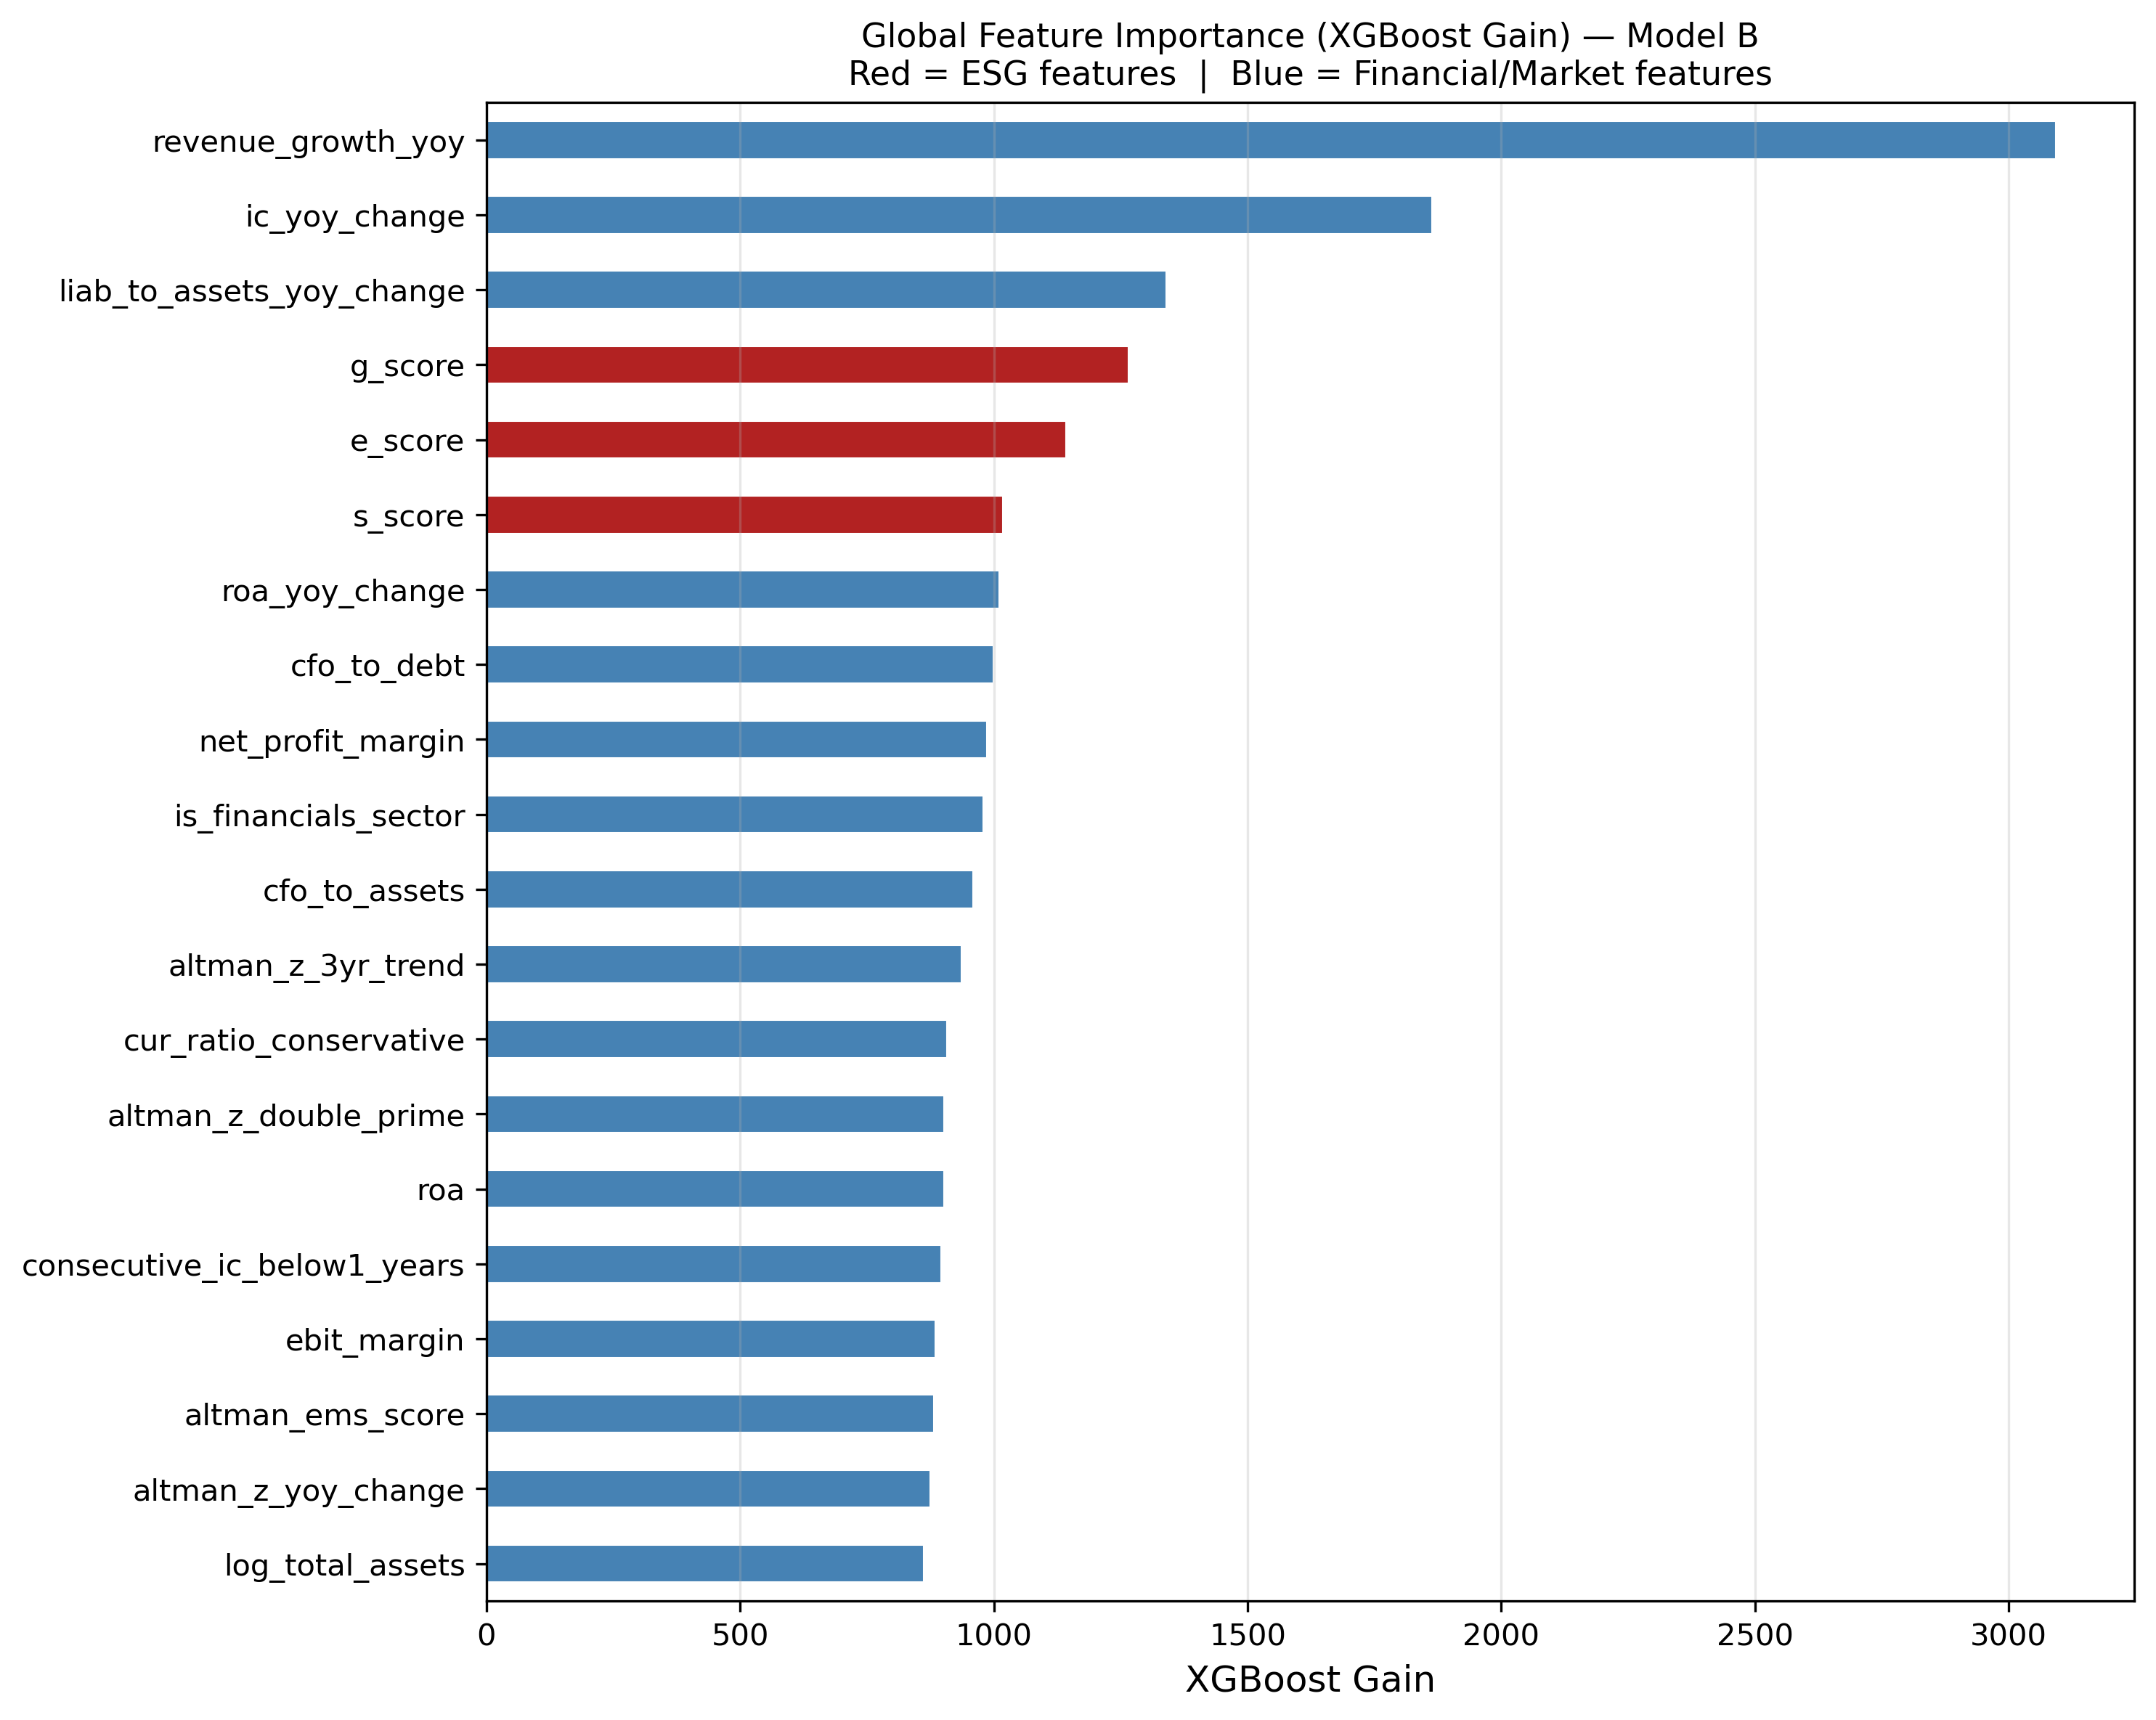
\includegraphics[width=\linewidth]{reports/figures/feature_importance.png}}
\caption{XGBoost native feature importance (gain) for Model~B. ESG features (red) command a substantial proportion of total information gain, corroborating the SHAP analysis.}
\label{fig_importance}
\end{figure}


%% ============================================================
%%  5. DISCUSSION
%% ============================================================
\section{Discussion}

\subsection{Answering the Research Questions}

\textbf{RQ1: Effect of circular-feature removal.}
After ablating six circular features and enforcing temporal separation, Model~A achieves an ROC-AUC of only 0.5348---barely above random chance and far below the 0.95+ scores commonly reported in studies that retain circular predictors. This result quantifies the degree to which published performance in distress prediction may reflect accounting identities rather than genuine forward-looking forecasting ability. The ablation creates the analytical conditions necessary for any orthogonal signal to become detectable.

\textbf{RQ2: ESG signal recovery.}
Model~B recovers the injected ESG signal, achieving a statistically significant ROC-AUC improvement of $+0.0774$ over Model~A ($p < 0.05$). The 5-stage signal diagnostic confirms that the ESG coefficient retains its correct sign and significance from the raw panel through to the out-of-time test set. SHAP analysis confirms that the three core ESG variables rank as the top three predictors, providing evidence of substantial ESG contributions consistent with the injected signal. The PDP shows a broadly decreasing relationship between \texttt{e\_score} and predicted distress probability, consistent with the protective signal encoded in the generation mechanism.

\textbf{RQ3: Class imbalance and threshold effects.}
At 0.2278\% prevalence, raw accuracy is decoupled from predictive utility. The five-classifier benchmark demonstrates this starkly: Random Forest achieves 99.58\% accuracy with zero positive-class recall, while Logistic Regression achieves 58.56\% accuracy with the highest recall (65.15\%). The threshold analysis shows that lowering the decision boundary to 0.30 captures 86.7\% of distress events, while raising it to 0.72 yields 98.20\% accuracy at the cost of detecting only 1.9\% of events. Threshold selection must be driven by the asymmetric cost structure of the application, not by accuracy optimization.

\subsection{Why Modest Performance is Informative}
The Model~B ROC-AUC of 0.6117 is deliberately modest compared to the near-perfect scores reported in studies that retain circular features. This modesty is a feature, not a limitation, of the experimental design. By removing the features that produce artificial inflation, the framework creates a realistic baseline against which the incremental contribution of ESG data can be measured. The result demonstrates that CRESTA can recover the injected ESG signal under the controlled non-circular experimental setting, even though the absolute magnitude of that signal is modest.

\subsection{The Accuracy Paradox}
The five-classifier benchmark provides a concrete illustration of the accuracy paradox under extreme class imbalance. Random Forest achieves the highest raw accuracy (99.58\%) by predicting 218 observations as positive, of which zero are true positives. Its balanced accuracy (49.91\%) is below random chance. Conversely, classifiers with lower accuracy (Logistic Regression at 58.56\%, XGBoost at 66.97\%) detect a meaningful fraction of the positive class. This underscores the importance of evaluating distress models with metrics that account for class prevalence---ROC-AUC, PR-AUC, balanced accuracy, and positive-class recall---rather than overall accuracy alone.

\subsection{Limitations}
Several limitations should be acknowledged.

\textbf{Synthetic data.} The injected ESG signal ($\gamma = -4.0$) represents an idealized, frictionless protective effect. Real-world ESG data may exhibit weaker, noisier, or sector-dependent relationships with distress risk. The 60,000-firm scale was chosen to ensure sufficient statistical power (264 test positives) at realistic annual distress rates, not to model actual firm counts.

\textbf{Bootstrap methodology.} The row-level percentile bootstrap may understate the confidence interval width because 57,196 of 58,677 test-set firms contribute two correlated annual observations. A firm-level cluster bootstrap would be a more conservative approach.

\textbf{No hyperparameter optimization.} All model hyperparameters were fixed without cross-validation or search. The XGBoost configuration may not be optimal, and different settings could change the absolute performance levels (though the relative ablation comparison remains valid).

\textbf{PDP non-monotonicity.} The partial dependence relationship between \texttt{e\_score} and predicted distress is broadly decreasing but not strictly monotonic, with local fluctuations attributable to the tree-based model's piecewise-constant boundaries.

\textbf{Generalizability.} Results are specific to the XGBoost architecture, the chosen hyperparameters, and the synthetic data-generating process. Other model architectures may recover the ESG signal with different efficiency. The synthetic findings do not automatically generalize to real-world corporate data.

\textbf{Coverage-flagged observations.} The 2,097 rows flagged for low feature coverage were retained in the feature matrix and participated in model training. In a production system, these rows might warrant exclusion or separate treatment.

\subsection{Practical Implications}
The CRESTA methodology provides a template for evaluating ESG integration in real-world distress models. Before deploying any ESG-augmented credit model, practitioners should verify that (1)~features circular with respect to the distress definition have been removed, (2)~temporal separation is enforced between features and labels, and (3)~model performance is assessed under metrics appropriate for the target prevalence. The threshold analysis demonstrates that operationally useful recall requires accepting a precision--false-alarm trade-off that cannot be optimized by accuracy alone.

We do not claim that the present system is deployment-ready. The synthetic validation establishes the pipeline's mechanical capacity to isolate an orthogonal signal; whether real-world ESG data provides a comparable signal remains an open empirical question.


%% ============================================================
%%  6. CONCLUSION AND FUTURE WORK
%% ============================================================
\section{Conclusion and Future Work}

This paper presented CRESTA, an evaluation framework for ESG-augmented corporate distress prediction that enforces temporal separation ($X_t \to Y_{t+1}$) and ablates features circular with respect to the distress definition. The framework was validated on a controlled synthetic testbed of 60,000 firms over 10~fiscal years, with a known ESG distress-protective signal ($\gamma = -4.0$) embedded in the data-generating mechanism.

Under strict out-of-time evaluation on 115,873 test observations (264 distress events, 0.2278\% prevalence), the financial-only model achieved near-random discrimination (ROC-AUC~$= 0.5348$), showing that circular-feature removal substantially reduces the artificial performance inflation observed when circular predictors are retained in this experimental setting. The ESG-augmented model achieved a statistically significant improvement (ROC-AUC~$= 0.6117$; $\Delta$AUC~$= +0.0774$, 95\% CI: [$+0.0455$, $+0.1080$]), and SHAP analysis confirmed that the three ESG variables ranked as the top global predictors. The 5-stage signal diagnostic verified that the injected coefficient survived all pipeline stages with correct sign and significance.

These results establish the pipeline's capacity for controlled signal recovery. They do not demonstrate real-world ESG predictive power, nor do they establish causal relationships between ESG performance and distress risk. The immediate trajectory for future research involves deploying the validated architecture on real-world Bloomberg financial data combined with mandated Indian Business Responsibility and Sustainability Reporting (BRSR) disclosures. Additional future work includes: implementing firm-level cluster bootstrap for more conservative statistical inference on panel data, conducting hyperparameter optimization via walk-forward cross-validation, and evaluating alternative model architectures to assess the generalizability of the ESG signal recovery.

\section*{Appendix A: Feature Engineering Dictionary}
The pipeline generates 44 engineered features across seven analytical blocks. After ablation of 6 circular features, 38 features serve as final model inputs. Representative definitions include:
\begin{itemize}
    \item \textbf{Size:} $\textit{Log\_Assets}_{t} = \ln(\textit{Total\_Assets}_t + 1)$; $\textit{Log\_MktCap}_t = \ln(\textit{Market\_Cap}_t + 1)$
    \item \textbf{Profitability:} $ROA_t = \textit{Net\_Income}_t / \textit{Total\_Assets}_t$; $\textit{EBIT\_Margin}_t = EBIT_t / \textit{Revenue}_t$
    \item \textbf{Leverage:} $\textit{Equity\_to\_Assets}_t = \textit{Total\_Equity}_t / \textit{Total\_Assets}_t$; $\textit{Debt\_to\_Assets}_t = \textit{Total\_Debt}_t / \textit{Total\_Assets}_t$
    \item \textbf{Liquidity:} $\textit{Current\_Ratio}_t = \textit{Current\_Assets}_t / \textit{Current\_Liabilities}_t$
    \item \textbf{Classical Composite:} Altman Z$''$ (double prime), adapted for non-manufacturing and emerging-market firms
    \item \textbf{Temporal Dynamics:} $\Delta ROA_{t} = ROA_t - ROA_{t-1}$; 3-year Altman Z trend; consecutive loss years; revenue growth
    \item \textbf{ESG:} \texttt{e\_score}, \texttt{s\_score}, \texttt{g\_score} (derived from latent \texttt{base\_esg} with additive noise); \texttt{carbon\_intensity} proxy
\end{itemize}

\begin{thebibliography}{00}
\bibitem{altman1968} E. Altman, ``Financial ratios, discriminant analysis and the prediction of corporate bankruptcy,'' \textit{The Journal of Finance}, vol.~23, no.~4, pp.~589--609, 1968.
\bibitem{ohlson1980} J. Ohlson, ``Financial Ratios and the Probabilistic Prediction of Bankruptcy,'' \textit{Journal of Accounting Research}, vol.~18, no.~1, pp.~109--131, 1980.
\bibitem{merton1974} R. Merton, ``On the Pricing of Corporate Debt: The Risk Structure of Interest Rates,'' \textit{The Journal of Finance}, vol.~29, no.~2, pp.~449--470, 1974.
\bibitem{jones2017} S. Jones, D. Johnstone, and R. Wilson, ``An empirical evaluation of the performance of binary classifiers in the prediction of credit ratings changes,'' \textit{Journal of Banking \& Finance}, vol.~56, pp.~72--85, 2015.
\bibitem{sculley2015} D. Sculley et al., ``Hidden Technical Debt in Machine Learning Systems,'' in \textit{Advances in Neural Information Processing Systems (NeurIPS)}, 2015.
\bibitem{rabanser2019} S. Rabanser, S. G\"{u}nnemann, and Z. Lipton, ``Failing Loudly: An Empirical Study of Methods for Detecting Dataset Shift,'' in \textit{NeurIPS}, 2019.
\bibitem{lundberg2017} S. Lundberg and S. Lee, ``A Unified Approach to Interpreting Model Predictions,'' in \textit{NeurIPS}, 2017.
\bibitem{chen2016} T. Chen and C. Guestrin, ``XGBoost: A Scalable Tree Boosting System,'' in \textit{Proc.\ 22nd ACM SIGKDD Int.\ Conf.}, 2016.
\bibitem{ke2017} G. Ke et al., ``LightGBM: A Highly Efficient Gradient Boosting Decision Tree,'' in \textit{NeurIPS}, 2017.
\bibitem{friede2015} G. Friede, T. Busch, and A. Bassen, ``ESG and financial performance: aggregated evidence from more than 2000 empirical studies,'' \textit{Journal of Sustainable Finance \& Investment}, vol.~5, no.~4, pp.~210--233, 2015.
\bibitem{bassen2006} A. Bassen and A. Kovachev, ``ESG-Performance and Corporate Value,'' \textit{SSRN Electronic Journal}, 2006.
\bibitem{lessmann2015} S. Lessmann, B. Baesens, H. Seow, and L. Thomas, ``Benchmarking state-of-the-art classification algorithms for credit scoring,'' \textit{European Journal of Operational Research}, vol.~247, no.~1, pp.~124--136, 2015.
\bibitem{barboza2017} F. Barboza, H. Kimura, and E. Altman, ``Machine learning models and bankruptcy prediction,'' \textit{Expert Systems with Applications}, vol.~83, pp.~405--417, 2017.
\bibitem{bellotti2009} A. Bellotti and J. Crook, ``Support vector machines for credit scoring and discovery of significant features,'' \textit{Expert Systems with Applications}, vol.~36, no.~2, pp.~3302--3308, 2009.
\end{thebibliography}

\end{document}
